\documentclass[a4paper]{report}

\usepackage{a4wide}
% To decrease the margins and allow more text on a page.

\usepackage{graphicx}
% To deal with including pictures.

\usepackage{enumerate}
% To provide a little bit more functionality than with LaTeX's default
% enumerate environment.

\usepackage{array}
% To provide a little bit more functionality than with LaTeX's default
% array environment.

\usepackage[parfill]{parskip}

\usepackage{float}

\usepackage{multicol}
% For if we want to put something in a multi column environment.

\usepackage[dutch]{babel}
% Use this if you want to write the document in US English. It takes care of
% (usually) proper hyphenation.
% If you want to write your answers in Dutch, please replace 'american'
% by 'dutch'.
% Note that after a change it may be that the first compilation of LaTeX
% fails. That is normal and caused by the fact that in auxiliary files
% from previous runs, there may still be a \selectlanguage{american}
% around, which is invalid if 'american' is not incorporated with babel.

\usepackage{amssymb}
% This package loads mathematical things like the fonts for the blackboard
% bold for the set of natural numbers.

\usepackage{amsmath}
% And some student asked me to include amsmath as well...

\usepackage{verbatimbox}
% For putting verbatim stuff into boxes.

\usepackage{tikz}
\usetikzlibrary{arrows}
\usetikzlibrary{positioning}
% The tikz package can be used to draw all kinds of diagrams.
% For instance parse trees and finite automata.

\usepackage[all]{xy}
% Instead of tikz you can also use xy to draw diagrams.


\usepackage{xspace}
% xspace can be used to let LaTeX decide whether a command should be followed
% by a space or not, depending on what follows.

% Replace the placeholders by your real names, student numbers and
% tutorial groups.
\newcommand{\norm}[1]{\left\lVert#1\right\rVert}

% Replace the placeholders by your real names, student numbers and
% tutorial groups.
\author{
	Matthijs Muis \\
	s1066918
}

\title{
	Statistiek \\
	Inleveropgave week 13 en 14
}

\begin{document}

\maketitle

\begin{abstract}
  Ter afronding van de huiswerkopgaven van het vak Statistiek zijn de laatste twee weken gewijd aan een wat groter project. Het doel is om een echte dataset te analyseren en hiervoor een lineair regressiemodel te formuleren en te fitten.

  Deze opdracht behandelt enkele van de in de opgave genoemde punten. Een aantal modellen wordt geformuleerd en deze worden vergeleken en getoetst met de technieken uit het vak. We zullen deze kwantitatieve resultaten ook verbinden met hun betekenis in de werkelijkheid. Andersom zullen we ons bij het formuleren van geschikte modellen laten leiden door redelijke aannames en hypothesen uit de `economische wetenschap'.
\end{abstract}

\newpage

\tableofcontents

\newpage

\chapter{Inleiding}

\section{Dataset}

  De gegeven dataset is een subset van de Fortune500 dataset uit 1986. Deze bevat $n = 52$ waarnemingen, met voor $i = 1, \dots ,n$ steeds een paar $(x_i,Y_i)$ waar $x_i \in \mathbb{R}^q$ voor $q = 4 + 2$, $Y_i \in \mathbb{R}$ met:
  
  \begin{align*}
  x_1 &= 1_{\text{[sector = "Finance"]}} &
  x_5 &= \text{assets} \\
  x_2 &= 1_{\text{[sector = "Energy"]}} &
  x_6 &= \text{marketval} \\
  x_3 &= 1_{\text{[sector = "Manufacturing"]}} &
  Y &= \text{sales} \\
  x_4 &= 1_{\text{[sector = "Retail"]}}
  \end{align*}
  
  Dit zijn twee continue variabelen en 4 dummy's, elke dummy representeert een level voor de categorische variabele \verb!sector!.
  
  Kwantitatief wordt de categorische data dus in binaire variabelen gerepresenteerd. Maar wanneer het ons uitkomt, roepen we in \verb!R! gewoon de categorische variabele aan. Sterker nog, hier is \verb!R! op gemaakt: \verb!marketval:sector! aanroepen in de command \verb!lm! zal bijvoorbeeld precies 4 interactievariabelen maken als producten $x_1x_6, \ x_2x_6, \ x_3x_6, \ x_4x_6$.
  
  De continue variabelen in de dataset zijn \verb!sales!, \verb!assets! en \verb!marketval!. Dit zijn de \emph{omzet}, het \emph{kapitaal} (in aandelen) en de \emph{marktwaarde} van het bedrijf. We doen net of de omzetten van de bedrijven realisaties zijn van een stochast $Y$ en de marktwaarde en het kapitaal vaste gegevens waar de omzet mogelijk door te verklaren is. Deze economische variabelen hebben de volgende betekenis:

\begin{enumerate}
  \item De \emph{(jaar)omzet} van een bedrijf is de winst die het bedrijf in een jaar heeft gemaakt.
  \item Het \emph{kapitaal} van een bedrijf is het totale geldbedrag dat de aandelenverkoop van het bedrijf heeft opgeleverd. Een bedrijf kan aandelen (assets) verkopen op de aandelenbeurs. Een koper van zo'n aandeel heet een aandeelhouder en het bezit van een aandeel betekent dat de aandeelhouder mag delen in de winst van het bedrijf middels een winstuitkering die \emph{dividend} heet. Voor het bedrijf is de aandeelhouder een investeerder en kan het kapitaal besteed worden aan hulpbronnen of uitbreidingen.
  \item De \emph{marktwaarde} van een bedrijf is de theoretische verkoopprijs van het bedrijf, dus een bod welke de markt vindt dat de eigenaar van het bedrijf redelijkerwijs zou kunnen accepteren voor de verkoop van het bedrijf, niet te hoog en niet te laag. Uiteraard is de marktwaarde niet een waargenomen variabele, maar moet deze geschat worden. Dit doen analisten op basis van allerlei data. Wij gaan ervan uit dat deze marktwaarde de `echte' marktwaarde is, voor ons is het dus wel een waarneming.
\end{enumerate}

  Tenslotte nog iets over de categorische variabele \verb!sector!: in de Fortune-500 dataset zit categorische variabele die de sector van het bedrijf aangeeft. Er zijn 4 sectoren of, in \verb!R!-jargon, \emph{levels}: \emph{Energy, Finance, Manufacturing} en \emph{Retail}. 
  
\subsection{Ori\"enterend Verdelingsonderzoek}
\label{Verdelingsonderzoek}
  Nu geven we eerst wat marginale verdelingen van deze variabelen met behulp van histogrammen. Deze plots zullen nog weinig informatie geven over het verband tussen de variabelen, maar het is handig om ze alvast bij de hand te hebben. Het maken van dit soort plots kan eenvoudig met de onderstaande commands in de command-line van \verb!R!.
  
  \begin{verbatim}
> barplot(summary(sector))
> hist(marketval)
> hist(sales)
> hist(assets)
  \end{verbatim}


  \begin{figure}[H]
  \label{covariaten marginaal}
  \begin{center}
  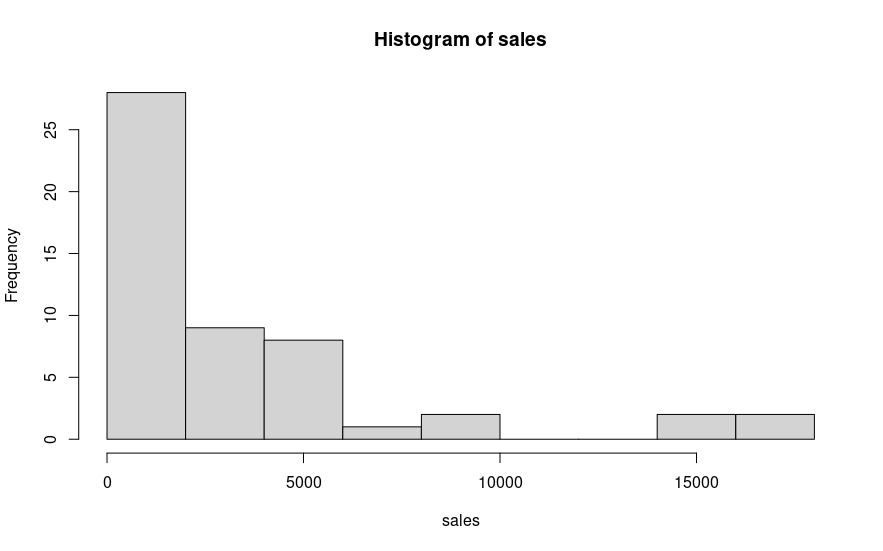
\includegraphics[width=.45\textwidth]{histSales.PNG}
  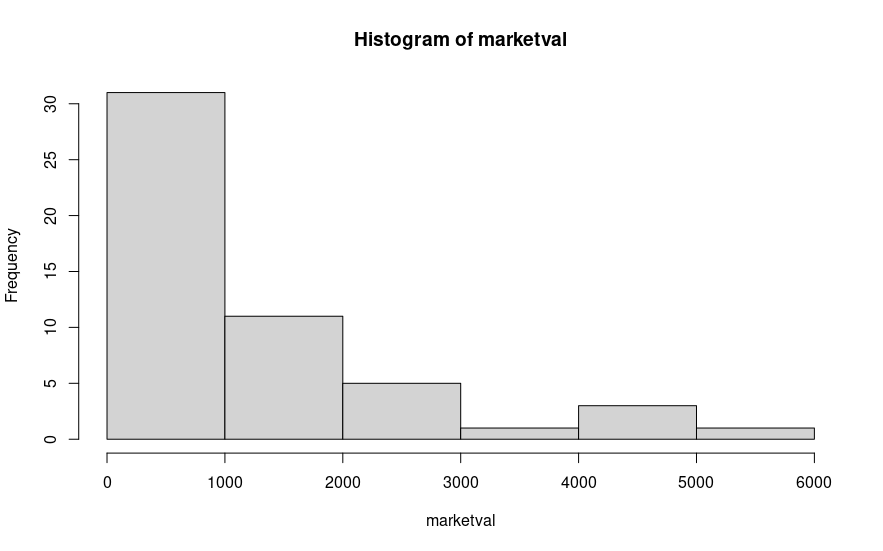
\includegraphics[width=.45\textwidth]{histMarketval.PNG}
  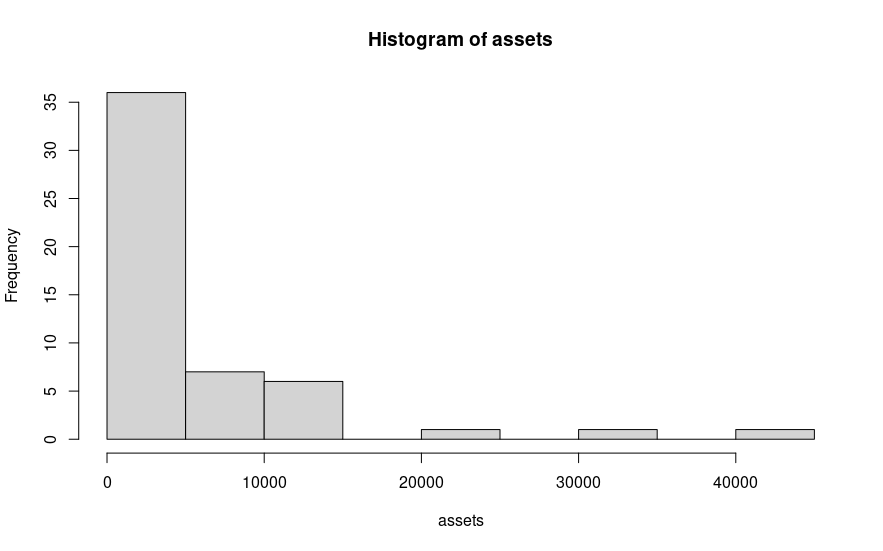
\includegraphics[width=.45\textwidth]{histAssets.PNG}
  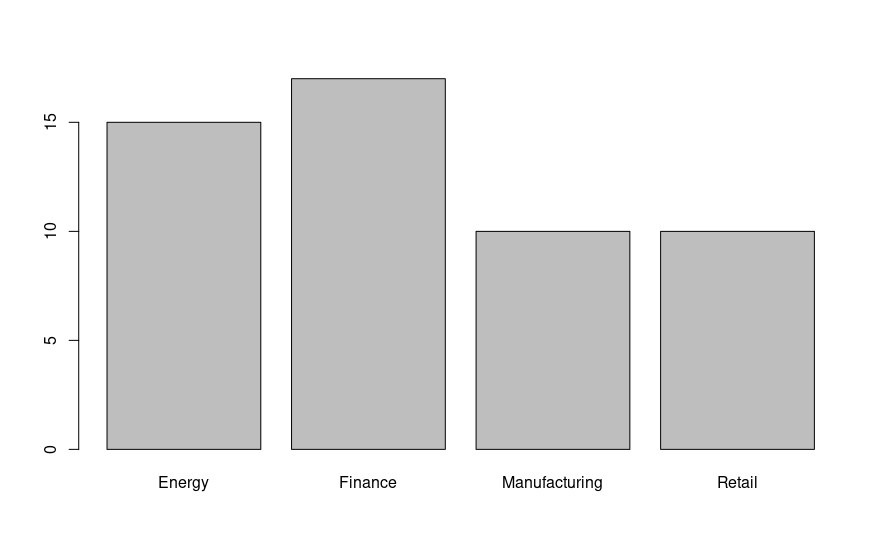
\includegraphics[width=.45\textwidth]{barSector.PNG}
  \end{center}
  \caption{De marginale verdelingen van de vier gegeven covariaten.}
  \end{figure}
  
  De bovenstaande plots geven als eerste indruk dat de financi\"ele variabelen erg scheef verdeeld zijn. Dit motiveert mogelijk een logaritmische transformatie van de financi\"ele data, waarover we hieronder nog uitgebreid zullen komen te spreken. De scheefheid is daarentegen geen onomstotelijk bewijs dat de logtransformatie noodzakelijk is. Het is bijvoorbeeld goed mogelijk dat de correlatie tussen de continue variabelen ervoor zorgt dat de residuen van het lineaire model t\' och normaal verdeeld blijken te zijn. Dit is waarom marginale verdelingen eigenlijk te weinig informatie bieden. We zullen ons vanaf nu voornamelijk bezig houden met de correlatie tussen de variabelen
  
  Over de precieze modelaannamen hebben we nog niet gesproken, zie hiervoor \ref{Model}. Het zal echter een lineair model worden met als verklaarde variabele \verb!sales! en als covariaten variabelen die alleen afhangen van \verb!assets!, \verb!marketval! en \verb!sector!. We verwachten in elk geval dat een groter kapitaal en een grotere marktwaarde gecorrelleerd zijn met een grotere omzet. Een bedrijf dat meer te besteden heeft zal meer investeringsmogelijkheden hebben en daardoor meer winst kunnen maken en daardoor waardevoller zijn dan een bedrijf dat minder winst maakt. 
  
  We gaan ons ori\"enteren op dit ruwe vermoeden door wat eendimensionale plots van de continue variabelen tegen elkaar, en de loggetransformeerde variabelen tegen elkaar. Steeds zijn de punten per sector gekleurd met een regressielijn erbij. In feite zijn we hier al twee heel eenvoudige lineaire model aan het fitten, namelijk \verb!sales ~ assets + sector! en \verb!log(sales) ~ log(marketval) + sector! (tenzij anders aangegeven \emph{inclusief} intercept).
  
  \begin{figure}[H]
  \label{2d scatterplots}
  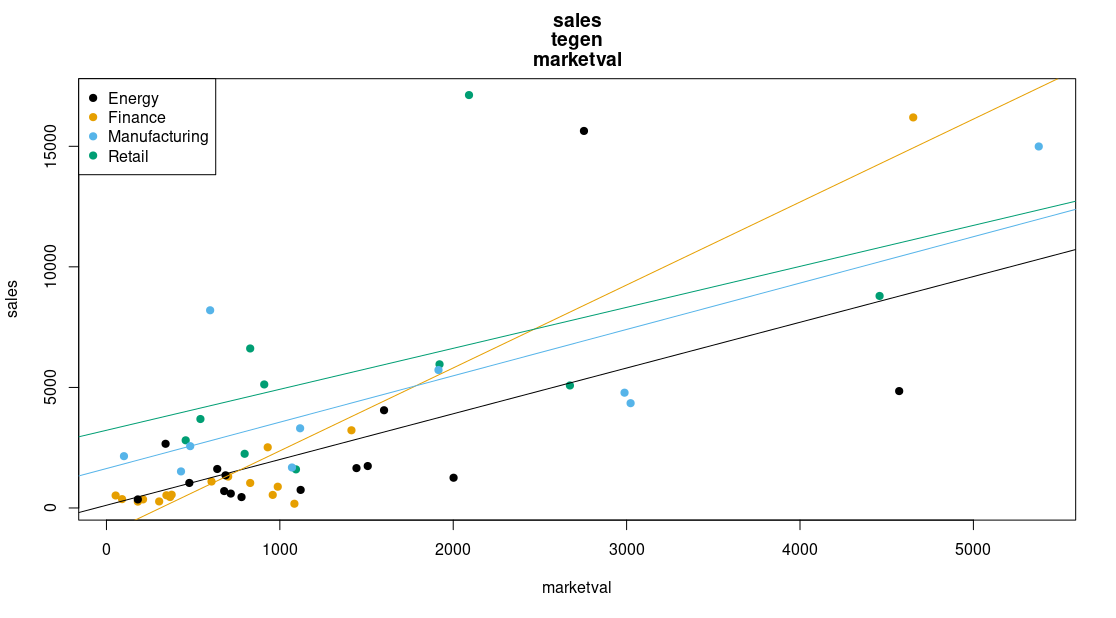
\includegraphics[scale=.45]{salesMarketval.PNG}
  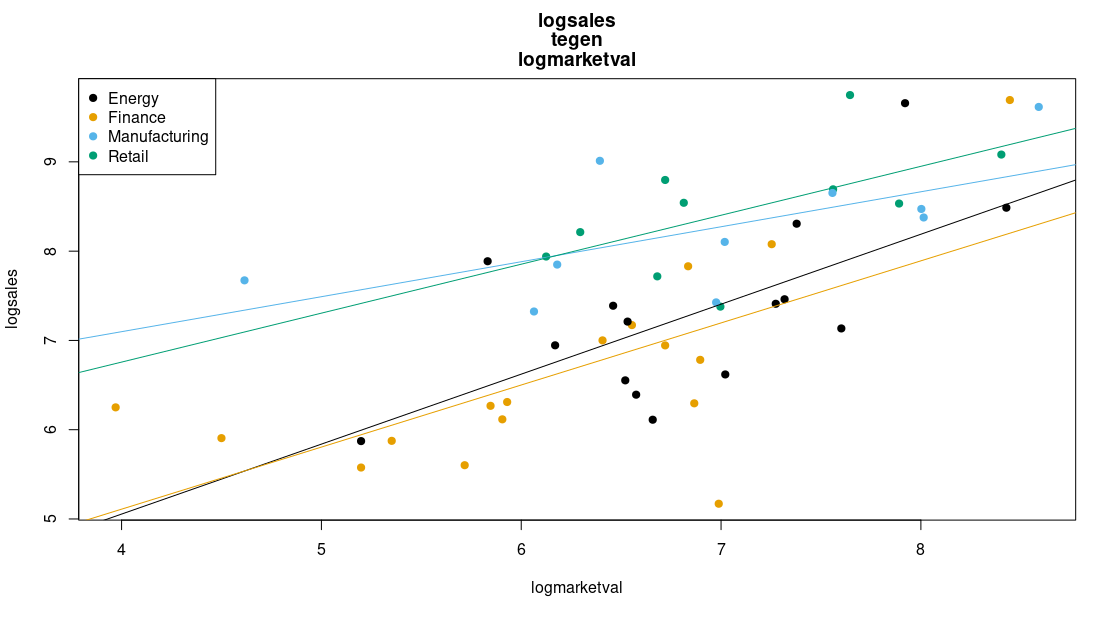
\includegraphics[scale=.45]{logsalesLogmarketval.PNG}
  \caption{Scatterplots van sales tegen marketval, sales tegen assets respectievelijk}
  \end{figure}
  \begin{figure}[H]
  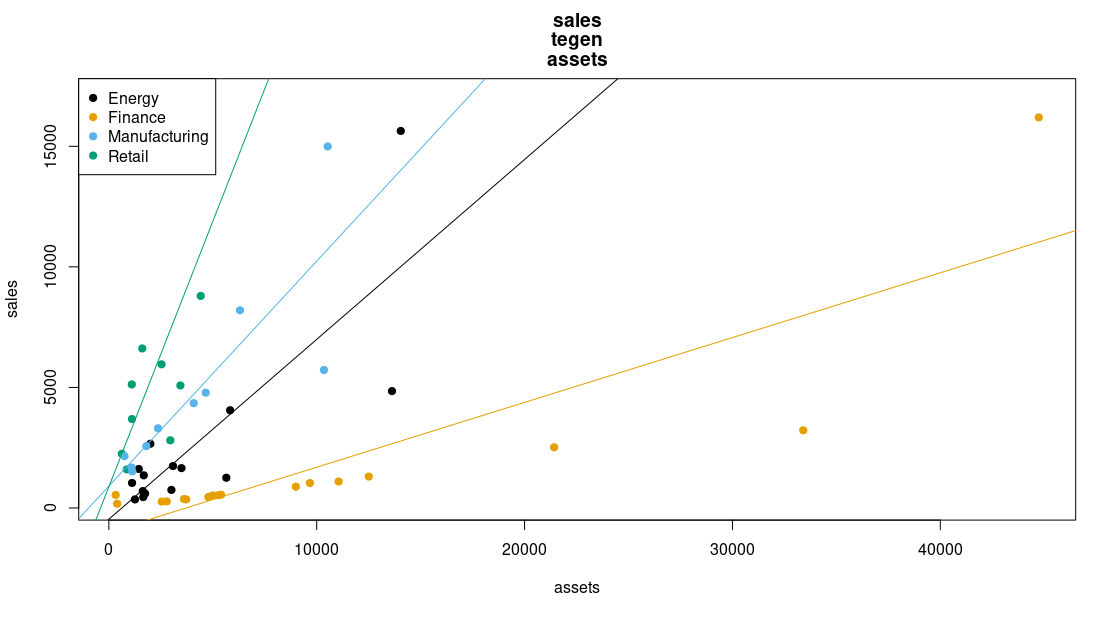
\includegraphics[scale=.45]{salesAssets.PNG}
  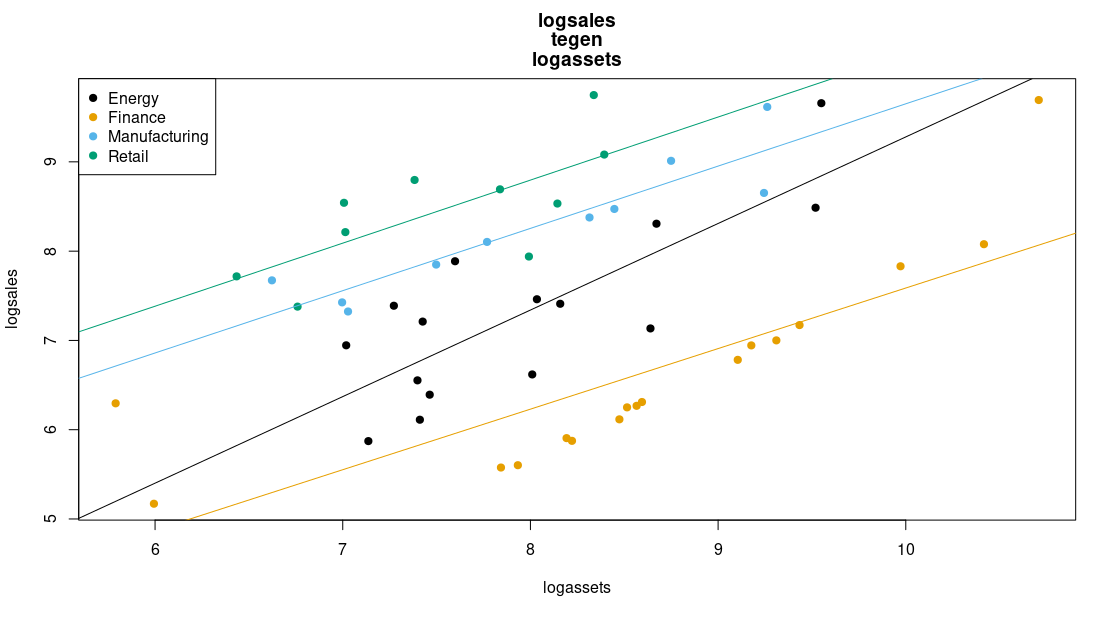
\includegraphics[scale=.45]{logsalesLogassets.PNG}
  \caption{Scatterplots van logsales tegen logmarketval, logsales tegen logassets respectievelijk.}
  \end{figure}
  
  In de bovenstaande figuur zien we een prachtinge scheiding optreden in bijvoorbeeld het vierde plot: De verschillende sectoren liggen in mooie lagen boven elkaar en lijken haast te smeken om een eigen intercept. Zonder het kleuren van de puntenwolk zou hier \' e\' en ongecorrelleerde hoop punten te zien zijn (tot kortgeleden stond op de voorgaande pagina een dergelijk plot met alleen zwarte puntjes: ik kon toen ook niet begrijpen dat het model uberhaupt iets verklaarde!). 
  
  Merk ook op dat deze verschillende intercepts in het log-getransformeerde model leiden tot verschillende hellingen en daardoor uitwaaierende regressielijnen in het `rauwe' model. Dit is een mooie visualisering van hoe een  redelijk homoskedastische log-variabele leidt tot een sterk heteroskedastische  `rauwe' variabele. Dat wordt een van onze motiveringen voor een log-transformatie.
  
\subsection{Voorbehoud} 
  We zien in alle plots een zwakke trend, maar vooral tussen \verb!logsales! en \verb!logmarketval!. Links zien we wederom scheefheid in de data, welke duidelijk leidt tot ongewenste \emph{heteroskedasticiteit} in beide modellen: de variantie van de errors is veel groter voor grotere waarden van de covariaten.
  
  Deze regressielijnen zijn in alle gevallen waarschijnlijk biased ten opzichte van het `werkelijke model': we verklaren bepaalde variantie van $Y$ met \' e\' en covariaat terwijl er mogenlijk sprake is van verklaring door nog een andere covariaat. Dat vertekent de sterkte van de rol van de zichtbare covariaat, zie H\ref{modelselectie} . $Y$ komt dan mogelijk tot stand door de optelsom van de twee covariaten, maar de enkelvoudige modellen `zien' echter voor zichzelf slechts \' e\' en van de twee (relevante?) covariaten en de effecten hiervan worden dan onzuiver geschat. Je zou kunnen zeggen dat de afbeeldingen in figuur \ref{2d scatterplots} steeds \' e\' en van de financi\"ele variabelen `wegmarginaliseren'.
  
  Om alle dimensies van de data in beeld te brengen (dat kan, de datapunten als hun continue variabelen bevinden zich in driedimensionale ruimte) heb ik ervoor gekozen zo'n 800 packages te installeren alvorens een 3d-scatterplot te maken. Het resultaat is een 3d-scatterplot. Enerzijds geeft dit de data volledig weer, anderzijds is een driedimensionale voorstelling in een tweedimensionale figuur moeilijk om helemaal in het juiste perspectief te zien. Ik heb 4 plots gemaakt, \' e\' en zonder schaling en \' e\' en met schaling van de assen.
 
  \begin{figure}[H]
  \label{3d scatterplots}
  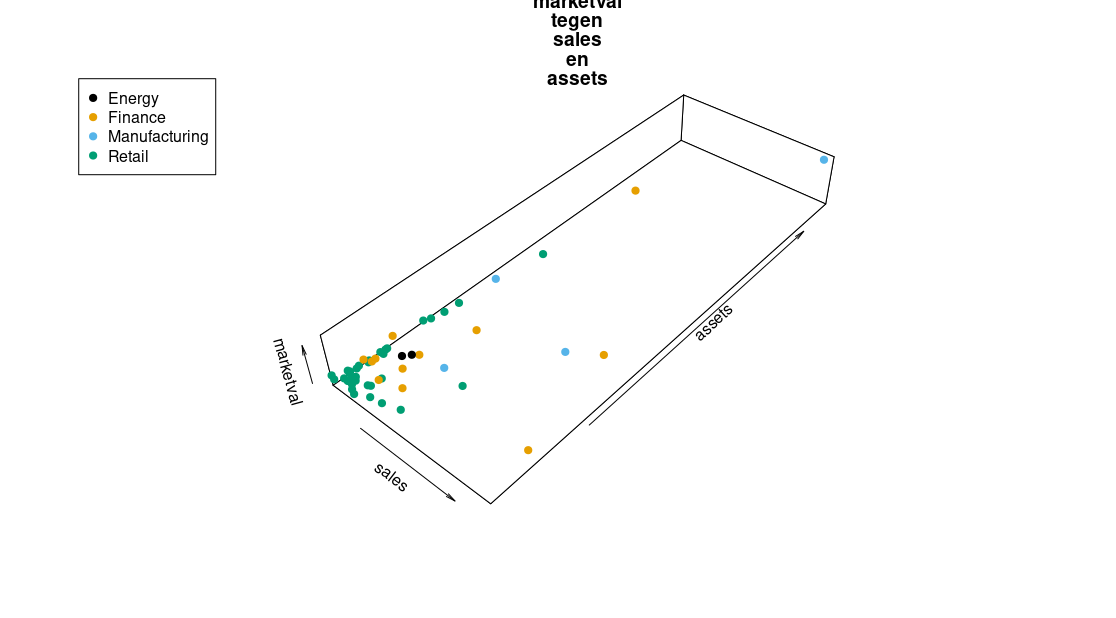
\includegraphics[scale=.45]{3dScatterUnscaled.PNG}
  \caption{Ongeschaalde scatterplot van sales tegen marketval en assets. Assets staat niet tegen de verticale as. Dat is hier niet zo erg, het gaat vooral om een visuele indruk van de clustering van de punten}
  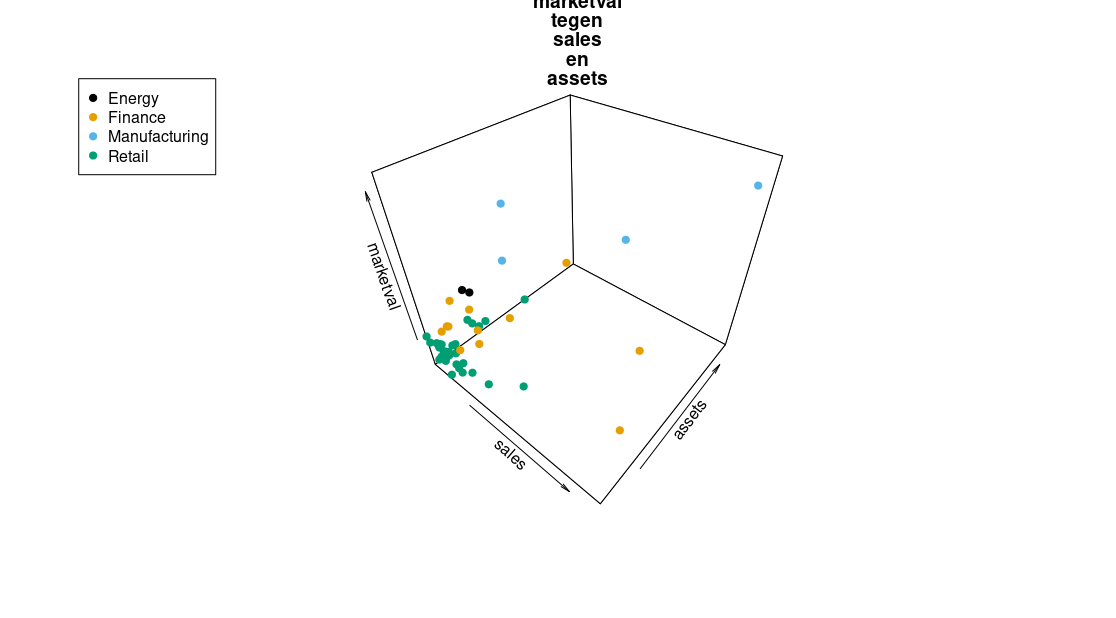
\includegraphics[scale=.45]{3dScatter.PNG}
  \caption{Geschaalde scatterplot van sales tegen marketval en assets.}
  \end{figure}
  \begin{figure}[H]
  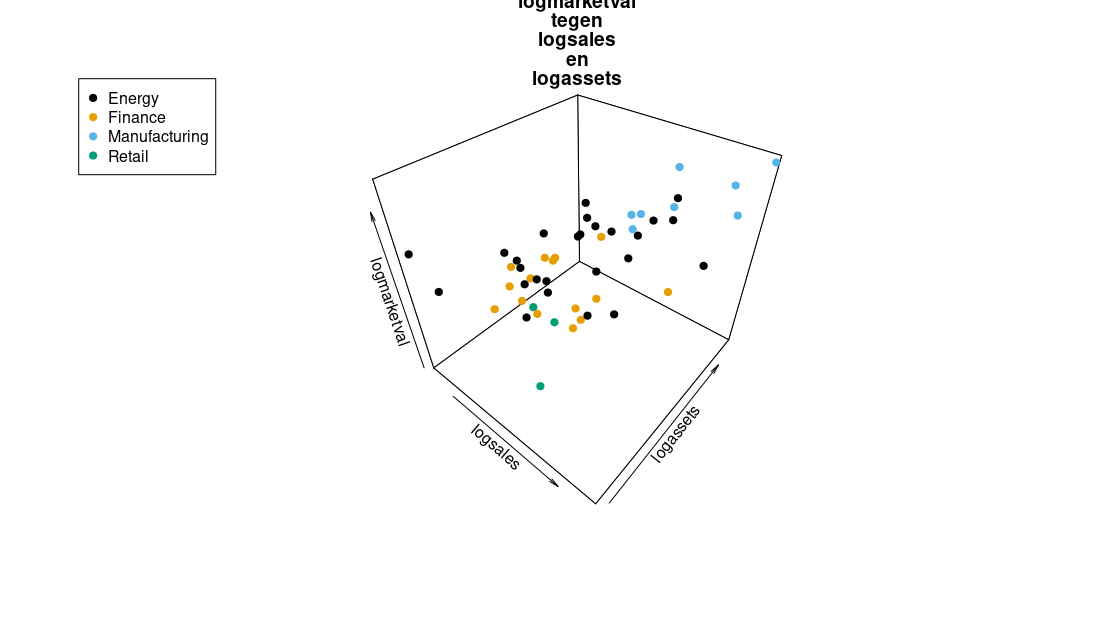
\includegraphics[scale=.45]{3dLogScatterUnscaled.PNG}
  \caption{Ongeschaalde scatterplot van logsales tegen logmarketval en logassets.}
  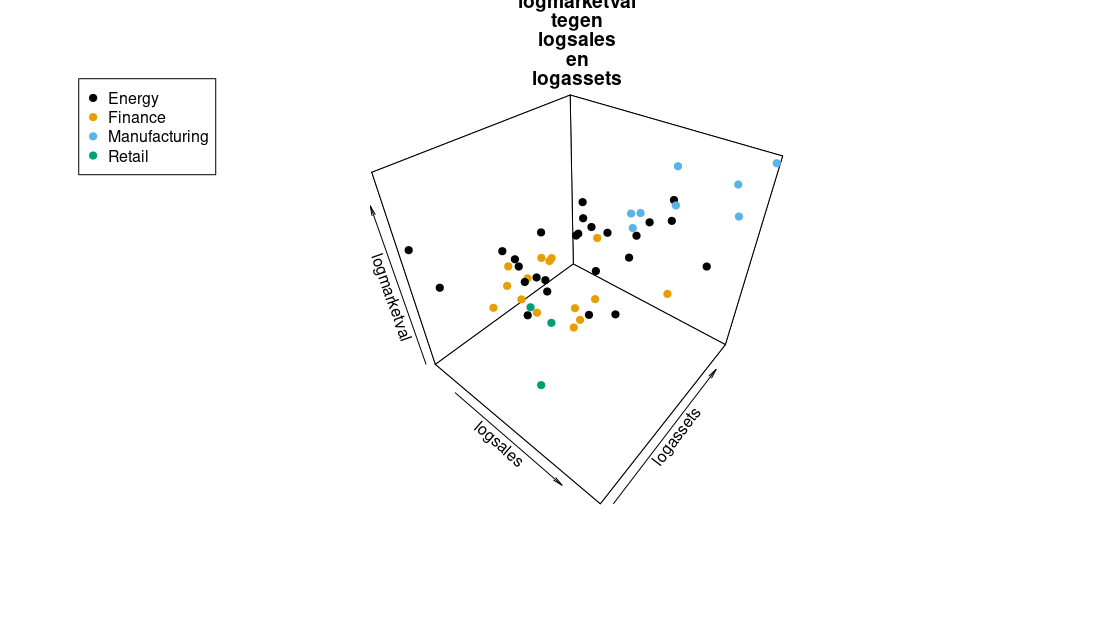
\includegraphics[scale=.45]{3dLogScatter.PNG}
  \caption{Geschaalde scatterplot van logsales tegen logmarketval en logassets. Door de logtransformatie zijn alle schalen ongeveer van dezelfde orde-grootte, daarom is slechts weinig verschil met de bovenstaande figuur te zien.}
  \end{figure}
  
\section{Model}  
\label{Model}
  We gaan een lineair model schatten met gronddata gegeven in de bovenstaande variabelen. Wanneer we over `covariaten' spreken, hebben we het over de covariaten hebben die op dat moment in dat model gekozen zijn. We doen de volgende modelaannamen voor een nog niet gekozen design-matrix $X \in \mathbb{R}^{n\times p}$ en de `stochastische' datavector $Y: \Omega \rightarrow \mathbb{R}^n$:
  
  \begin{align}
  Y &= X\beta + \varepsilon \\
  \varepsilon &\sim \mathcal{N}(0,\sigma^2I)
  \end{align}
  
  Later gaan we dit model uitbreiden door ons af te vragen of de varianties van de errors niet per level van \verb!sector! apart moeten worden geschat. Deze uitbreiding ziet er, formeel geformuleerd, als volgt uit:
  
  \begin{align}
  Y &= \begin{pmatrix} X_{\text{m}}  \\ X_{\text{f}} \\ X_{\text{r}} \\ X_{\text{e}} \end{pmatrix}\beta + \varepsilon \\
  \varepsilon &\sim \mathcal{N}(0,
  \begin{pmatrix} 
  \sigma_{\text{m}}^2I & & & \\ 
  & \sigma_{\text{f}}^2I & & \\ 
  & & \sigma_{\text{r}}^2I & \\
  & & & \sigma_{\text{e}}^2I \\
  \end{pmatrix})
  \end{align}
  
  We partitioneren de designmatrix $X$ dus in 4 blokken waar we de waarnemingen die een bepaalde sector (m, f, r, e) hebben groeperen in \' e\' en blok. Corresponderend daarmee wordt de covariantiematrix van $\varepsilon$ een diagonaalmatrix met ter hoogte van ieder blok diagonaalelementen die worden geparametriseerd door de variantie $\sigma_{\text{sector}}^2$ horend bij die sector.

\section{Onderzoeksvragen}
  In dit hoofdstuk gaan we enkele vragen formuleren bij de data die interessant kan zijn bij het analyseren van verbanden in de dataset. Aan de hand van deze vragen kunnen we verdelingsonderzoek verrichten en daarna een aantal kandidaatmodellen formuleren die ons zinvol lijken.
  
  Ik heb me bij het formuleren van de vragen gebaseerd op eigen ingeving alsook op de suggesties uit de opdracht.  
  
  De vraag is voornamelijk welk lineair model het beste $Y$ verklaart. Die vraag is niet altijd objectief. Een heel groot lineair model zal altijd meer variantie in de afhankelijke variabele opvangen omdat de kolomruimte van de designmatrix groter is dan een subset van dit model, en zal dus altijd beter presteren op de \emph{gegeven} data. De vraag is daarom ook of de opgenomen effecten wel significant bijdragen.
  
  \begin{enumerate}
  \item Is een $\log$-transformatie voor de financi\"ele variabelen zinvol?
  
  \item Is er significante variatie in conditionele verdelingen van \verb!sales! of anders \verb!logsales! afhankelijk van \verb!sector!? In woorden, is het zinvol om de effecten van de continue variabelen per sector te schatten?
  
  \item Zie in dit opzicht ook suggestie 6: is het zinvol om de \emph{variantie} in de errors per categorie te schatten? Dit is een uitbreiding op het model uit \ref{Model}. De precieze formulering is dan, of $\varepsilon \sim \mathcal{N}(0,\Sigma^2)$ met $\Sigma^2$ een diagonaalmatrix, maar nu op de diagonaal is $(\Sigma^2)_{ii} = \sigma^2_{\text{sector}}$, welke nog afhangt van de \verb!sector! van rij (datapunt dus) $X_{i-}$. 
  
  Dit vermoeden kunnen we toetsen met een nieuwe toetsingsstatistiek die gegeven is in de opgave. Op het eerste gezicht lijkt het zoeken naar bepaalde varianties lastiger te implementeren, maar vergeet niet dat \verb!R! gebouwd is voor dit soort vragen.
  
  Tenslotte merken we op dat de hypothese van deze toets, $H_0:\sigma_1=\sigma_2=\sigma_3=\sigma_4$ tegen $H_1: \sigma_1
  \neq \sigma_2 \neq \sigma_3 \neq \sigma_4$, steeds binnen een model geformuleerd wordt. Fitten we meerdere modellen, dan moeten we deze toets ook voor deze verschillende modellen apart uitvoeren.
  \end{enumerate}
  
\section{Constanten}
\label{constanten}

\begin{align*}
n &= 52 \quad \text{steekproefgrootte} & \alpha = 0.05 \quad \text{betrouwbaarheidsniveau} \\
\end{align*}
  
\chapter{$\log$-transformatie voor financi\"ele data}
\section{Ecomische motivatie voor $\log$-transformatie}
\label{economische motivatie}
  Er bestaat een heldere motivatie voor het $\log$-transformeren van financi\"ele data. In het geval van financi\"ele data zijn afhankelijkheden veelal ratio en niet additief. Beschouw immers de volgende (zeer eenvoudige) modellen voor de omzet van een bedrijf, afhankelijk van het kapitaal:

\begin{align}
  \text{sales} = \alpha + \beta \cdot \text{assets} \\
  \text{log(sales)} = \alpha + \beta \cdot \text{log(assets)}
\end{align}
  (N.B. deze modellen corresponderen met de twee onderste trendlijnen in figuur 1.2)
  
  Het is intu\"itief aansprekend dat wanneer het kapitaal van een bedrijf met 5\% stijgt, de marktwaarde met een evenredig (niet per se gelijk) percentage zal toenemen. Dit correspondeert met een lineaire verschuiving van $\log(\text{sales})$ (n.l. met $\log(1.05)$), en een daaruit volgende lineaire verschuiving van $\log(\text{sales})$ (n.l. met $\beta \log(1.05)$). Een uitspraak als `wanneer een retailbedrijf in kapitaal verdubbelt, zal de omzet met 50\% toenemen' correspondeert met een $\beta = \log(2)/\log(1.5)$.
  
  Wat het ongetransformeerde lineaire model postuleert, is veel minder aannemelijk. Dit verband houdt namelijk in dat per extra 1\$ in omzet de marktwaarde met $\beta$\$ zal stijgen. Maar niet voor elk kapitaalniveau zal elke extra dollar direct omgezet worden in $\beta$ extra dollar winst, om het maar even grof te formuleren. Deze toename per extra dollar noemen economen de `marginale omzet' (wij noemen het de afgeleide), en een van de centrale aannamen in de economie is juist de wet van `diminishing returns', dus dat deze marginale omzet afneemt. 
  
  Een motivatie voor deze wet is eenvoudig: bij toename van het kapitaal naar een steeds groter bedrag, zullen toch andere variabelen - zoals begrensde afzetmogelijkheden - beperkingen opleggen aan de winst. Neem bijvoorbeeld MacDonalds: dit bedrijf kan met meer kapitaal weliswaar meer restaurants openen, meer reclamezuilen huren en in nog goedkopere productiemethoden voor burgers investeren en met nog meer kwantumkorting aardappel(meel) inkopen om er frietjes van te maken, uiteindelijk is er een grens aan het aantal bezoeken per persoon per dag en dus aan de verkoop van producten. Het kan dus niet anders of de `(kapitaal $\mapsto$ winst)-functie' zal ergens beginnen te krommen naar een asymptoot.
  
  
  Het is moeilijk om deze kromming waar te nemen in de gegeven data, dus voor deze subsection zal het helaas blijven bij wat economisch gefilosofeer. De volgende motivatie voor de $\log$-transformatie is statistisch van aard en zullen we op rigoreuze wijze hard maken.
  
  Tenslotte moeten we ook de mogelijkheid overwegen om alleen de verklarende of alleen de verklaarde variabele te transformeren. Dit heeft echter geen zinvolle economische interpretatie en is daardoor moeilijk te rechtvaardigen. Bovendien worden twee verschillende eenheden met elkaar in verband gebracht: namelijk geld en ratio's van geld. Dat is ook niet erg logisch. Het komt in praktijk dan ook nooit voor.
 
\section{Statistische motivatie voor de $\log$-transformatie} 
\subsection{Heteroskedasticiteit}
  Een andere motivatie van het nemen van $\log$-transformaties heeft meer te maken met de verdeling van het logaritme van financi\"ele data. Financi\"ele data blijkt in praktijk heel scheef verdeeld te zijn. Wederom is dat logisch, want in een groot bedrijf met veel kapitaal passen veel kleine bedrijfjes met weinig kapitaal. De verhouding bedrijven met `groot kapitaal' tot bedrijven `klein kapitaal' is daardoor scheef. 
  
  Deze observatie deden we al toen we keken naar de marginale verdelingen van de financi\"ele variabelen in onze dataset (zie 1.1). We zagen de scheefheid terugkomen in de uitbijters in het scatterplot van de ongetransformeerde data.
  
  Deze uitbijters zijn desastreus voor de gepostuleerde modelaanname van \emph{homoskedasticiteit}, d.w.z. de variantie van de residuen is constant en niet gecorrelleerd met de grootte van de covariaten. Immers, als het logaritme van elke financi\"ele variabele, zeg $Z$ een vaste verdeling volgt, zoals een normale verdeling, dan volgen de financi\"ele variabelen de verdeling van $\exp(Z)$. De $\exp$-functie kromt sterk naar boven voor grotere waarden van $Z$, dus bij kleine variatie van $Z$ rond een bepaald punt $x$ is variatie van $\exp(Z)$ klein voor kleine waarden van $x$ en juist heel groot voor grote waarden van $x$. dus als $\text{log(sales)} = \alpha + \beta \cdot \text{log(assets)}$ voldoet aan homoskedasticiteit, dan $\text{sales} = \alpha + \beta \cdot \text{assets}$ z\' eker niet!
  
  We kunnen echter veel rigoureuzere uitspraken doen over deze financi\"ele variabelen met statistische toetsen. Ik wil zelfs beweren dat de marginale verdelingen van de $\log$s van de financi\"ele data inderdaad normaal zijn. Nu gaan we een Kolgomorov-Smirnov-toets uitvoeren om dit te toetsen voor de marginale verdelingen van \verb!assets!, \verb!marketval! en \verb!sales!.
  
\subsection{Kolgomorov-Smirnov-toets op normaliteit van logassets, logmarketval en logsales}  
\label{KS-toets}
  Het idee achter de KS-toets is bekend uit \emph{Inleiding in de Statistiek}. Voor $H_0: F = F_0, \ H_1: F \neq F_0$: zij $T$ de grootste absolute afwijking tussen de empirische verdelingsfunctie van de data en de nulverdeling $F_0$, dan volgt $T$ een bekende verdeling en verwerpen we voor $T$ groot genoeg.
  
  Het probleem met de KS-toets, welke ook in dat boek wordt behandeld, is dat men $F_0$ eigenlijk graag wil kiezen op basis van geschatte parameters n\' adat men de data heeft waargenomen. Wij willen nu bijvoorbeeld controleren of \verb!assets! een normale verdeling bezit, en als $F_0$ willen we graag de verdeling kiezen die als gemiddelde en variantie het waargenomen steekproefgemiddelde en de waargenome variantie van \verb!assets! bezit. Dit mag niet, omdat $F_0$ een vaste verdeling moet zijn die niet mag afhangen van de data dus ook niet van de schatters $\bar{X_n}$ en $S^2_X$.
  
  Een uitbreiding van de KS-statistiek $T^*$ (zie wederom \emph{Inleiding in de Statistiek}) is gegeven voor het tupel van hypothesen $H_0: F \in \mathcal{F}_0, \ H_1: F \not \in \mathcal{F}_0$. Hierbij is $\mathcal{F}_0$ een familie van verdelingsfuncties (bijvoorbeeld een locatieschaalfamilie), je zou kunnen zeggen een model. $T^*$ is nu de grootste absolute deviatie tussen de empirische verdelingsfunctie en de verdelingsfunctie die geparametriseerd is door de maximum-likelihoodschatters van de parameters. In praktijk zijn deze voor een normale verdeling $\overline{X_n}$ en $S_X$ en geeft dit de volgende toetsingsgrootheid:

  \begin{equation}
    T^* = \sup_{x\in \mathbb{R}} | \mathbb{F}_n(x) - \Phi(\frac{x-\overline{X_n}}{S_X})|
  \end{equation}  	
	
   We zijn nu ge\"interesseerd in de verdeling van $T^*$ onder de nulhypothese, zodat we bij zeer incompatibele waarden van $T^*$ de nulhypothese kunnen verwerpen en een $p$-waarde kunnen geven. Merk echter op dat de verdeling van $T^*$ in zijn geheel niet triviaal is. We zouden deze kunnen simuleren, maar ook dan is de vraag met welk element (welke normale verdeling dus) van $\mathcal{F}_0$ we dit zouden moeten doen. Immers hangt de verdeling van $T^*$ misschien wel af van de ware parameter van de normale verdeling? 
   
   Op p.146 van \emph{Inleiding in de Statistiek} staat gelukkig dat de verdeling van $T^*$ hetzelfde is onder ieder element van $\mathcal{N}$. We nemen dus een standaardnormale verdeling en bepalen met behulp van simulatie de nulverdeling van $T^*$: we nemen een simulatiesteekproef van 1,000,000.

  Vervolgens bepalen we de KS-test statistiek met de ingebouwde functie in \verb!R!. Dit doen we voor \verb!assets!, \verb!marketval! en \verb!sales!, en dus ook voor \verb!logassets!, \verb!logmarketval! en \verb!logsales!. Dit zijn, zoals de namen al zeggen, de $\log$-getransformeerde variabelen.
  
  Kortheidshalve is de \verb!R!-code uit de tekst gelaten.
  
  \begin{figure}[H]
  \begin{center}
  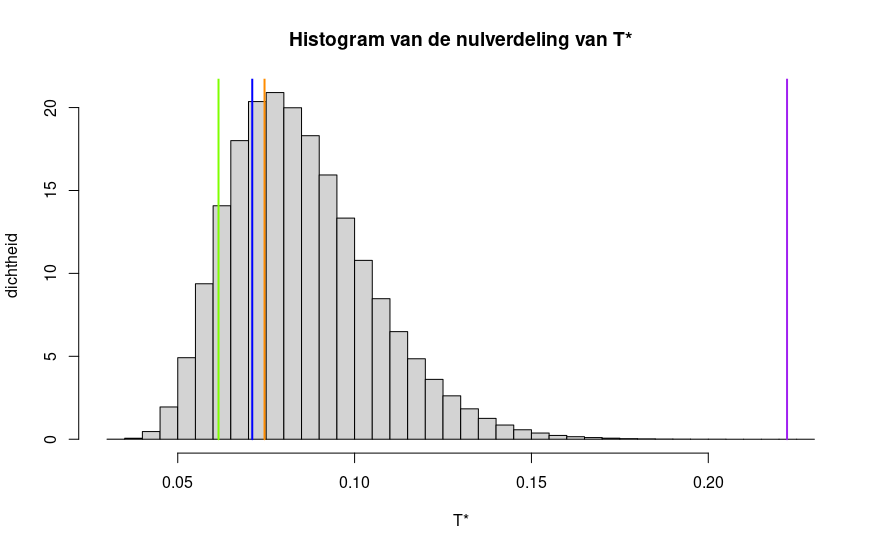
\includegraphics[scale=.5]{KSTestLog.PNG}
  \begin{multicols}{2}
  \begin{verbatim}
 > pvalue(Tlogsales)
[1] 0.663722
> pvalue(Tlogassets)
[1] 0.897291
> pvalue(Tlogmarketval)
[1] 0.734819

> pvalue(Tsales)
[1] 1e-06
> pvalue(Tassets)
[1] 0
> pvalue(Tmarketval)
[1] 0
  \end{verbatim}
  \end{multicols}
  \end{center}
  \caption{De gesimuleerde nulverdeling van $T^*$. In de grafiek zijn ook de werkelijke waarden van $T^*$ gegeven voor de dataset: groen: logassets, blauw: logmarketval, oranje: logsales, paars, rood, magenta: overlappen elkaar, dit zijn de ongetransformeerde variabelen. We zien dat deze zeer incompatibel met $H_0$ zijn. Onderstaand de $p$-waarden bij de toets.}
  \end{figure}   
  
  We kunnen met grote zekerheid zeggen dat de `raw' data niet normaal verdeeld is: de $p$-waardes zijn heel klein. Daarentegen is het best aannemelijk (niet verwerpbaar) dat de getransformeerde data wel normaal verdeeld is. Merk overigens op dat dit niet hoeft te betekenen dat de residuen van $Y$ na enige fit dat ook zijn. Toch bleek uit de plots onder \ref{Verdelingsonderzoek} dat voor de raw data zichtbare heterogeneiteit te zien was. Om deze, en de hierbovenstaande theoretische motivatie is besloten de regressiemodellen alle te fitten voor de $\log$ van de financi\"ele data.

\chapter{Theorie over Lineaire modellen en Modelselectie}
\label{modelselectie}
  Uitgaande van het model uit \ref{Model} is er veel statistische theorie rondom het schatten en uitvoeren van toetsen op deze modellen. Wij benoemen hier enige relevante theorie die helpt bij het interpreteren van de summary's uit het voorgaande hoofdstuk. Ook vormen we wat nieuwe theorie voor de vraag, hoe te toetsen of een (collectie) regressor(s) aan het model kan worden toegevoegd of moet worden weggelaten.

\section{Schatten}
  \verb!R! schat lineaire modellen door de schatter $\hat{\beta}$ zodanig te kiezen dat de kwadratensom van de residuen, $\norm{Y-X\hat{\beta}}^2$, geminimaliseerd wordt. Dit heet de kleinste-kwadratenschatter. Onder de aanname van normaal verdeelde errors/residuen met een constante variantie (homoskedasticiteit) is deze schatter equivalent met de maximum-likelihood schatter.
  
  Deze schatter heeft een directe formule, welke gelijk is aan de berekening van de vector $\hat{\beta}$ die een lineaire combinatie $X\hat{\beta}$ maakt die precies de loodrechte projectie van $Y$ op $V$, de colspace van $X$, is.
  
  Een afleiding van de formule is te vinden in \emph{Inleiding in de Statistiek}. Hier staat hij:
  
  \begin{equation}
  \label{kleinste kwadraten schatter}
  \hat{\beta} = (X^tX)^{-1}X^tY
  \end{equation}
  
  Deze schatter is zuiver onder de modelaannames.

\section{Restricted Models}
  Het lastige van modellen fitten, is dat schattingen voor parameters in een model niet goed met de werkelijke parameterwaarden overeen zullen komen, wanneer een gepostuleerd model niet overeenkomt met het werkelijke `model'. Bij lineaire modellen ligt dit `overeenkomen met het werkelijke model' vaak in de keuze om een bepaalde variabele wel of niet op te nemen in het model.
  
  Stel dat het `werkelijke model' van de volgende vorm is:
  
  \begin{align}
  Y &= X_0\beta_0 + X_1\beta_1 + \varepsilon \\
  \varepsilon &\sim \mathcal{N}(0,\sigma^2I)
  \end{align}
  
  In andere woorden, deel in \ref{Model} de designmatrix op in blokken: $X = \begin{pmatrix} X_0 & X_1 \end{pmatrix}$, en de parameter in twee corresponderende stukken: ${\beta = \begin{pmatrix} \beta_0 \\ \beta_1 \end{pmatrix}}$. 
  
  We kunnen het `wel of niet ertoe doen' en het `wel of niet opnemen in het model' van variabelen uit $X$ nu als volgt formuleren:
  
  \begin{enumerate}
  \item \label{restricted} Als we $X_1$ niet opnemen in het model, maar deze w\' el relevant is, dan schatten we een zogeheten `restricted model'. De aanname van het model is dus $\beta_1 = 0$. Noem de schatter van $\beta_1$ onder deze aanname $\hat{\beta}_R$.
  
  \item \label{te uitgebreid} Als we $X_1$ wel opnemen in het model, maar in werkelijkheid is deze niet relevant, i.e. $\beta_1 = 0$ in het werkelijke model, dan schatten we $\beta_0$ en $\beta_1$ dus beide terwijl we eigenlijk alleen $\beta_0$ hoeven te schatten, en wel op basis van alleen $X_0$.
  \end{enumerate}
  
  Intu\"itief is duidelijk dat \ref{restricted} leidt tot een onzuivere schatting van $\beta_0$, doordat we mogelijk een effect van $X_1$ onterecht toeschrijven aan $X_0$. Evenzo is duidelijk dat in \ref{te uitgebreid}, als $X_1$ geen effect heeft in het werkelijke model, we ook naar verwachting $\hat{\beta}_1$ als 0 zullen schatten en $\hat{\beta}_0$ als $\beta_0$, dus dat de schatters wel zuiver zullen blijven. Maar ook is duidelijk dat we extra variantie introduceren in het schattingsproces, doordat we nu rekening moeten houden met de extra toegevoegde random regressors $X_1$.
  
  We zullen deze intu\"itie nu wiskundig hard maken, door de schatters $\hat{\beta}_R$ uit \ref{restricted} en $\hat{\beta}_0$ uit \ref{te uitgebreid} uit te drukken in de ware parameters:
  
\subsection{Onterecht Restricted}
\label{onterecht restricted}
  \begin{align*}
  \hat{\beta}_R &= (X_0^tX_0)^{-1}X_0^tY \\ 
  &= (X_0^tX_0)^{-1}X_0^t(X_0\beta_0 + X_1\beta_1 + \varepsilon) \\
  &= \beta_0 + (X_0^tX_0)^{-1}X_0^tX_1\beta_1 + (X_0^tX_0)^{-1}X_0^t\varepsilon
  \end{align*}
  
  We zien dat deze schatter een verwachte waarde heeft van $\beta_0 + (X_0^tX_0)^{-1}X_0^tX_1\beta_1$. Er is dus een onzuiverheid $(X_0^tX_0)^{-1}X_0^tX_1\beta_1$, welke groter wordt naarmate $\beta_1$ verder afwijkt van $0$. Dat is intu\"itief ook logisch, want het restricted model doet onterecht de aanname dat $\beta_1=0$; hoe fouter deze aanname, hoe fouter onze schatter wordt.
  
  Men kan echter ook aantonen dat de matrix $(X_0^tX_0)^{-1}X_0^t$ de error $\varepsilon$ terugschaalt. Dit impliceert dat de onzuivere schatter $\hat{\beta}_R$ voor $\beta_0$ wel weer minder variantie heeft dan $\hat{\beta}$ (aangezien we het hier over stochastische vectoren hebben, betekenent dit dat $\text{var}\hat{\beta}_0 - \text{var}\hat{\beta}_R$ positief semidefiniet is). Dit betekent dat als $\beta_1 \approx 0$, dan wordt het interessant om het restricted model te overwegen omdat dit effici\"enter is, hoewel biased. De onzuiverheid $(X_0^tX_0)^{-1}X_0^tX_1\beta_1$ zal dan namelijk ook klein zijn en hiertegen weegt de gereduceerde variantie mogelijk wel op.
  
\subsection{Onterecht te Uitgebreid}
\label{onterecht te uitgebreid}
  Schrijf eerst de afbeelding $\beta \mapsto \beta_0: \mathbb{R}^{p_0+p_1} \rightarrow \mathbb{R}^{p_0}$ als matrix $K = \begin{pmatrix} I_{p_0} & 0 \end{pmatrix}$. 
  \begin{align*}
  \hat{\beta}_0 &= K\hat{\beta} = K(X^tX)^{-1}X^tY \\ 
  &= K(X^tX)^{-1}X^t(X_0\beta_0 + \varepsilon) \\
  &= K(X^tX)^{-1}X^t(X\begin{pmatrix} \beta_0 \\ 0 \end{pmatrix} + \varepsilon) \\
  &= K \begin{pmatrix} \beta_0 \\ 0 \end{pmatrix} + K(X^tX)^{-1}X^t\varepsilon \\
  &= \beta_0 + K(X^tX)^{-1}X^t\varepsilon 
  \end{align*}
  
  De verwachting hiervan is precies $\beta_0$, dus de schatter is zuiver. Maar wel zagen we onder \ref{onterecht restricted} dat voor $\beta_1 =0$ de schatter $\hat{\beta}_R$ minder variantie heeft en geen onzuiverheid meer heeft, zodat deze effici\"enter is. Als $X_1$ dus geen rol speelt in het werkelijke model, is het beter om het ook weg te laten uit het geschatte model. Het is dus ook onwenselijk om het model te groot te maken (zogeheten \emph{kitchen-sink regression}, gootsteenregressie).
  
\subsection{Niet-geneste modellen}
\label{niet genest}

  Dit geval is eigenlijk een veralgemenisering van de voorgaande twee. Nu hebben we een partitie van $X = \begin{pmatrix} X_0 & X_1 & X_2 \end{pmatrix}$ in 3 blokken waarbij bijvoorbeeld de modellen zijn gekozen:
  
  \begin{enumerate}
    \item $Y = X_0\beta_0 + X_1 \beta_1$
    \item $Y = X_1\beta_1 + X_2 \beta_2$
  \end{enumerate}
  
  We zien dat de covariaten nu geen subset meer vormen. De reden om dit te vergelijken kan bijvoorbeeld zijn dat een overkoepelend model (d.w.z. een model met variabelen uit 1 en 2) niet erg verklarend blijkt te zijn, maar dat deze twee modellen elk voor zich goede verklaring lijken te bieden. Hoe nu te toetsen welk van de twee modellen `beter' is? Een standaard $F$-toets gaat alleen over geneste modellen, waarbij een model groter is in de zin dat er variabele zijn toegevoegd aan het andere model. De $F$-toets is hier dus niet toepasbaar. 
  
  Er zijn alternatieve toetsen, die in bijvoorbeeld H8 van \emph{Inleiding in de Statistiek} worden gegeven. Denk hierbij aan Aikake's Informatie Criterion. We zullen ons hier niet te lang mee bezighouden. We zullen namelijk zien dat het model \ref{Basale Model} erg goed verklaard en daarom toch meestal als basis wordt genomen voor verdere uitbreidingen.
  
\section{Toetsen voor modeluitbreidingen en -restricties}

  We willen nu toetsen of een model, dat (in regressors) een subset van een ander model is, significant slechter verklaard dan het grotere model. Oftewel, dat het gerechtvaardigd is om de extra variabelen van het grote model `erbij te nemen' omdat deze echt iets lijken te verklaren. 
  
  We toetsen dan of de parameters $\beta_1$, het verschil van de modellen gelijk aan nul kunnen worden gekozen. De hypothesen zien eruit als:
  \begin{align*}
  H_0 &: \beta_1 = 0 & H_1 &: \beta_1 \neq 0
  \end{align*}
  
  We voeren verder de volgende namen in: $p_0$ is de lengte van $\beta_0$, $p$ de lengte van $\beta$ ($p_1$, de lengte van $\beta_1$, is dan $p-p_0$). Verder is $V_0$ de kolomruimte van $X_0$ en $V$ de kolomruimte van $X$ (Dus is $V = V_0 + V_1$ waarbij $V_1$ de kolomruimte van $X_1$ is). Vanwege de eis dat $X$ volle rang heeft, volgt dat $\dim V_0 = p_0$, $\dim V = p$. 
  
  Er zijn twee gevallen mogelijk: $\beta_1$ heeft lengte 1, dus het gaat om het toevoegen van slechts \' e\' en co\"effici\"ent, of $\beta_1$ bestaat uit meerdere co\"effici\"enten. In het eerste geval is een $t$-toets uit te voeren, waarmee we al redelijk bekend zijn. In het tweede geval is de $F$-toets een bekende toets. Het blijkt overigens dat de $F$-toets in het geval $p_1 = 1$ equivalent is aan de $t$-toets.
  
\subsection{$t$-toets}
\label{t toets}
  In het meest algemene geval kunnen we een $t$-toets uitvoeren op het model voor een $a^t \in \mathbb{R}_p$ en $c \in \mathbb{R}$ en een paar hypothesen van de vorm:
  \begin{align*}
  H_0 &: a^t\beta = c & H_1 &: a^t\beta \neq c
  \end{align*}
  
  Of een eenzijdige variant hierop. Het idee is dat men een eendimensionale parameter $a^t\beta$ cre\"eert. Met behulp van de schatter $\hat{\beta}$, welke vanwege normaliteit van $\varepsilon$ zelf een normale verdeling volgt, kan men een (onder $H_0$ $t$-verdeelde) statistiek construeren uit $S^2 = SS_{\text{res}}/(n-p)$ en $\hat{\beta}$.
  
  \begin{equation}
  \label{t-statistic}
  T = \frac{a^t\hat{\beta}-c}{\sqrt{S^2a^t(X^tX)^{-1}a}}
  \end{equation}
  
  Onder $H_0$ geldt $T \sim t_{n-p}$, de afleiding hiervan is in het college gegeven.
  
\subsection{$F$-toets}
\label{F toets}
  Voor de vraag of een deelvector zoals $\beta_1$ van \emph{hogere dimensie dan 1} misschien weleens $0$ zou kunnen zijn, is de $t$-toets niet geschikt. We hebben namelijk een toets van de vorm $H_0: \beta_1 = 0$ tegen $H_1:\beta_1 \neq 0$, wat niet in termen van \' e\' en lineaire afhankelijkheid $a^t\beta_1 = c$ kan worden geschreven.
  
  We bekijken een andere statistiek. We berekenen hiertoe volgende statistieken:
  
  \begin{align}
  \norm{\Pi_{V_0}Y - \Pi_{V}Y}^2\\
  \norm{Y - \Pi_{V}Y}^2
  \end{align}   
  
  Waarbij $\Pi_V$ een projectie op $V$ voorstelt. Deze projectieruimtes staan loodrecht op elkaar en zijn daarom wegens het lemma van Cochran als volgt verdeeld:
  
  \begin{align*}
  \norm{\Pi_{V_0}Y - \Pi_{V}Y}^2/\sigma^2 &\sim \chi_{n-p_0} &
  \norm{Y - \Pi_{V}Y}^2/\sigma^2  &\sim \chi_{n-p}
  \end{align*}
  
  Wegens de stelling van Pythagoras (in $n$-dimensionale Euclidische ruimte) volgt bovendien:
  
  \begin{equation*}
  \norm{Y - \Pi_{V_0}Y}^2  = \norm{Y - \Pi_{V}Y}^2 + \norm{\Pi_{V_0}Y - \Pi_{V}Y}^2
  \end{equation*}
  
  Maar dan kunnen we herschrijven in termen van $SS_{\text{res},H_0}$ en $SS_{\text{res}}$:
  
  \begin{align*}
  \norm{\Pi_{V_0}Y - \Pi_{V}Y}^2 &= SS_{\text{res},H_0} - SS_{\text{res}} &
  \norm{Y - \Pi_{V}Y}^2 &= SS_{\text{res}}
  \end{align*}
  
  We maken nu een toetsingsstatistiek:
  
  \begin{equation}
  F = \frac{SS_{\text{res},H_0} - SS_{\text{res}}}{SS_{\text{res}}} \cdot \frac{n-p}{p-p_0}
  \end{equation}
  
  Omdat we denkbeeldig in de teller en de noemer van de eerste breuk beide door $\sigma^2$ kunnen delen, en de teller en noemer dan onafhankelijk van elkaar een standaard $\chi^2$-verdeling volgen, bereiken we dat $F$ onder $H_0$ een verdeling volgt die alleen afhangt van $n,p$ en $p_0$. Deze verdeling is de $F$-verdeling, en met de kritieke waarden van deze verdeling kunnen we de $F$-toets maken.

\chapter{Basale Model en Uitbreidingen met Interactietermen}

  Dit hoofdstuk geeft een overzicht van de (nu nog homoskedastische, d.w.z. $\sigma^2$ overal gelijk) modellen die geformuleerd worden in dit werkstuk. We geven eerst het meest eenvoudige model. Daarna breiden we dit model uit door interactietermen toe te voegen. Stapsgewijs zullen we deze modellen met elkaar vergelijken door middel van geschikte toetsen (zoals de $F$-toets als behandeld onder \ref{F toets}).
  
\section{Basale Model}
\label{Basale Model}
  Dit model heeft 6 parameters, namelijk een intercept, twee voor de regressors \verb!logassets! en \verb!logmarketval! en nog drie voor de dummy's die corresponderen met de overige sectoren. Als basislevel van \verb!sector! wordt ``Energy'' genomen, dat doet \verb!R! zelf (alfabetische volgorde van de levels) (en welk level het baselevel wordt is niet zo relevant, zolang we dit maar voor elk ander model consistent hetzelfde kiezen, anders wordt het moeilijker de modellen te vergelijken). De summary ziet er als volgt uit:
  
  \begin{figure}[H]
  \begin{verbatim}
lm(formula = logsales ~ logmarketval + logassets + sector)

Residuals:
    Min      1Q  Median      3Q     Max 
-0.8064 -0.3430 -0.1136  0.2910  1.1818 

Coefficients:
                    Estimate Std. Error t value Pr(>|t|)    
(Intercept)          0.67694    0.66809   1.013 0.316244    
logmarketval         0.27718    0.09436   2.937 0.005157 ** 
logassets            0.59310    0.09065   6.543 4.43e-08 ***
sectorFinance       -0.85830    0.21671  -3.961 0.000258 ***
sectorManufacturing  0.90871    0.21757   4.177 0.000130 ***
sectorRetail         1.34954    0.22439   6.014 2.76e-07 ***
---
Signif. codes:  0 ‘***’ 0.001 ‘**’ 0.01 ‘*’ 0.05 ‘.’ 0.1 ‘ ’ 1

Residual standard error: 0.5327 on 46 degrees of freedom
Multiple R-squared:  0.8151,	Adjusted R-squared:  0.795 
F-statistic: 40.56 on 5 and 46 DF,  p-value: 9.248e-16
  \end{verbatim}
  \caption{De summary van de fit. De geschatte co\"effici\"enten staan in de kolom `Estimate'. }
  \end{figure}  
  
\subsection{Individuele significantie van continue variabelen}

  \verb!R! heeft de $p$-waarden voor de $t$-toetsen voor de hypothesen $H_0:\beta_i = 0 \quad H_1:\beta_i \neq 0$ al voor ons uitgevoerd en in de summary gezet. Deze zijn te zien onder \verb!Pr(>|t|)!. We zien dat voor elke co\"effici\"ent behalve de intercept de nulhypothese wordt verworpen en dat deze dus significant is: er is dus voor elke covariaat een statistisch significant effect op \verb!logsales!.
  
  We hoeven ons dus niet af te vragen of het nodig is een van de continue variabelen te verwijderen, want de $t$-toetsen voor \verb!logmarketval! en \verb!logassets! uit de display geven hier direct antwoord op. Voor de categorische variabele zeggen de $t$-toetsen niet zo veel: een $t$-toets geeft namelijk alleen voor d\' ie dummy aan of die significant niet-0 is of niet. Of alle dummy's tegelijk niet-0 zijn, kan alleen worden getoetst met een $F$-toets.

  Dat de intercept niet aantoonbaar significant is, is jammer. Maar we kunnen deze variabele (de 1-kolom) niet verwijderen uit het model. Immers vormt hij ook de base-level voor de categorische variabele \verb!sector!, namelijk voor base-level Energy. Het kan niet goed ge\"interpreteerd worden als we deze base-level uit het model trekken. Dat zou dan betekenen dat Energy standaard intercept 0 krijgt, en de andere `modellen per sector' wel een eigen intercept krijgen.
  
\subsection{$F$-statistiek in toets tegen intercept-model}
  Tenslotte vermelden we dat de \verb!F-statistic! zoals deze in de summary verschijnt, de berekende $F$-statistiek is voor de toets $H_0: \forall i>1 \ \beta_i = 0$ tegen $H_1: \exists i>1 \ \beta_i \neq 0$. Deze toetst dus de verbetering van dit model tegen het model dat alleen de intercept heeft. Ik heb dit even nagerekend, en deze komt bijna volledig overeen:
  
\begin{verbatim}
# F-test tegen model met alleen intercept (intercept-model)
fit0 = lm(formula = logsales ~1)
p0 = 1
p = 6
n = 52
f = (sum(fit0$residuals^2) - sum(fit31$residuals^2))
  /(sum(fit31$residuals^2))*(n-p)/(p-p0) # F-statistic

pval = 1 - pf(f, p-p0,n-p)

> f 
[1] 40.55567
> pval
[1] 8.881784e-16
\end{verbatim}
  
  De $p$-waarde komt niet helemaal overeen met de summary, maar dit is te wijten aan afrondingsfouten (we werken dan ook in orde-grootte van \verb!e-15!, daar zijn afrondingsfouten relatief groot). De $p$-waarde van deze $F$-toets is echt heel klein: we verwerpen dus dat dit model niet beter verklaart dan het interceptmodel. Dus dit model kunnen we als basis nemen voor verdere uitbreidingen.
  
\subsection{$F$-toets tegen model zonder sector}
  Is de aparte intercept per sector een goed idee? Als we kijken naar de gekleurde figuren onder \ref{Verdelingsonderzoek}, zouden we zeggen van wel. De datapunten lagen, met name in \verb!logsales ~ logmarketval! in mooie lagen boven elkaar. Zonder aparte intercept leek \verb!logsales! bovendien weinig gecorrelleerd met \verb!logmarketval!. We kunnen dit hard maken met een $F$-toets:
  
  \begin{figure}[H]
  \begin{verbatim}
fit1 = lm(formula = logsales ~ logmarketval + logassets)
p0 = 3
p = 6
n = 52
f = (sum(fit1$residuals^2) - sum(fit31$residuals^2))/(sum(fit31$residuals^2))*(n-p)/(p-p0) # F-statistic
pval = 1 - pf(f, p-p0, n-p)

> f 
[1] 28.79964
> pval
[1] 1.237201e-10
  \end{verbatim}
  \end{figure}
  
  Wow! Wat een significantie! We zien dat ons vermoeden bevestigd wordt: de sectoren een eigen intercept geven is een goede keuze. We maken het model dus zeker niet kleiner. In de volgende paragrafen gaan we wel wat uitbreidingen overwegen.
  
\section{Effect van logassets per sector}
\label{uitbreiding logassets:sector}
  Een redelijke veronderstelling is dat de effecten van het kapitaal op de omzet verschilt van sector tot sector. Dit heeft te maken met de werking van bedrijven in verschillende sectoren: 

  \begin{enumerate}
    \item Retailbedrijven hebben over het algemeen een kleinere asset-base ten opzichte van hun omzet, omdat een groot deel van hun kosten zit in de inkoop van producten die ze weer verkopen. Denk aan een supermarkt: het gros van het kapitaal zit in producten die (soms binnen een dag) verkocht (moeten) worden. Kengetallen als inventory turnover zijn in deze sector heuse prestatiematen.
    
    \item Aan de andere kant van het spectrum zijn er financi\"ele bedrijven als banken, verzekeraars, die geld verdienen uit investeringen en rente daarop. Om risico's te dekken hebben zij juist expres een grote `buffer'. Centrale banken hanteren zelfs strikte kengetallen die het eigen vermogen van banken, pensioenfondsen ten opzichte van hun uitstaande investeringen groot moet houden (`vereiste eigen vermogen')
\end{enumerate} 
  
  We vangen dit verschil in effecten door per sector een eigen co\"effici\"ent voor \verb!logassets!. Dit introduceert dus 4 interactietermen in het model, in \verb!R! genoteerd met \verb!logassets:sector!. We behouden de co\"effici\"ent \verb!logassets!, zodat R een baselevel invoert, n.l. wederom Energy. Op die manier blijven de kolommen van de oude designmatrix van \ref{Basale Model} een subset van de designmatrix van het nieuwe model. Dat stelt ons in staat om later een $F$-toets uit te voeren en deze modellen zodoende te vergelijken. De summary ziet er als volgt uit:
  
  \begin{figure}[H]
  \begin{verbatim}
lm(formula = logsales ~ logmarketval + logassets + sector + logassets:sector)

Residuals:
    Min      1Q  Median      3Q     Max 
-0.8612 -0.3284 -0.1205  0.3494  1.1689 

Coefficients:
                              Estimate Std. Error t value Pr(>|t|)   
(Intercept)                   -0.31932    1.42442  -0.224  0.82368   
logmarketval                   0.28535    0.10436   2.734  0.00904 **
logassets                      0.71131    0.20166   3.527  0.00101 **
sectorFinance                 -0.01916    1.74507  -0.011  0.99129   
sectorManufacturing            3.14723    2.09009   1.506  0.13943   
sectorRetail                   2.83930    2.42794   1.169  0.24867   
logassets:sectorFinance       -0.10583    0.21698  -0.488  0.62820   
logassets:sectorManufacturing -0.28072    0.26061  -1.077  0.28742   
logassets:sectorRetail        -0.19146    0.31445  -0.609  0.54580   
---
Signif. codes:  0 ‘***’ 0.001 ‘**’ 0.01 ‘*’ 0.05 ‘.’ 0.1 ‘ ’ 1

Residual standard error: 0.5431 on 43 degrees of freedom
Multiple R-squared:  0.8203,	Adjusted R-squared:  0.7869 
F-statistic: 24.54 on 8 and 43 DF,  p-value: 1.147e-13
  \end{verbatim}
  \caption{De summary van de fit. De geschatte co\"effici\"enten staan in de kolom `Estimate'. }
  \end{figure}
  
  We zien ook dat alle variabelen uit \ref{Basale Model} terug te vinden zijn in dit model. Er zijn maar 3 variabelen toegevoegd.
  
  Het is zorgwekkend om te zien dat de $t$-toetsen voor individuele significantie bijna alle leiden tot een zwakke conclusie, en dat zelfs met heel hoge $p$-waarden. In dit model zijn alleen nog \verb!logmarketval! en \verb!logassets! individueel significant. 
  
  Hoe kan het dat ook de variabelen die in het model \ref{Basale Model} significant waren, dat nu niet meer zijn? Dit heeft te maken met de introductie van meer variabelen. Zoals besproken onder \ref{te uitgebreid} leidt het tot een hogere variantie van de schatter $\hat{\beta}$ wanneer deze langer wordt gemaakt. Gevolg hiervan is ook een grotere standard error en dit leidt tot kleinere $t$-values (je deelt door een grotere \verb!SE!). Dus dat de $t$-toets minder snel verworpen wordt. Je `betaalt' voor de extra vrijheid van het model door nu minder sterke uitspraken te kunnen doen over de parameters. Deze trade-off is karakteriserend voor de statistiek.
  
  De $F$-statistiek voor dit model tegen het model uit \ref{Basale Model} is berekend door:
  \begin{figure}[H]
  \begin{verbatim}
fit32 = lm(
  formula = logsales ~ logassets + logmarketval + sector + logassets:sector
  )

p0 = length(fit31$coefficients)
p = length(fit32$coefficients)
n = length(logsales)

f = (sum(fit31$residuals^2) - sum(fit32$residuals^2))
    /(sum(fit32$residuals^2))*(n-p)/(p-p0)
pval = 1 - pf(f, p-p0, n-p)

> f 
[1] 0.4183782
> pval
[1] 0.7407098
  \end{verbatim}
  \caption{De R-code om de $F$-statistiek te berekenen en de $F$-test uit te voeren tussen de twee modellen \ref{Basale Model} en \ref{uitbreiding logassets:sector}. We trekken de zwakke conclusie bij niveau 0.05.}
  \end{figure}
  
  We zien een erg kleine waarde van de $F$-statistiek, en corresponderend hiermee een zeer grote overschrijdingskans. Deze is groter dan het gekozen niveau $\alpha = 0.05$ (zie \ref{constanten}), dus we verwerpen $H_0$ niet: conclusie is dat het kleinere model \ref{Basale Model} niet minder verklarend is dan dit model. We laten dit model dus verder links liggen.
  
\section{Effect van logmarketval per sector}
\label{uitbreiding logmarketval:sector}
  Het volgende wat we ons kunnen afvragen is of het effect van marktwaarde op de omzet verschilt per sector. Een verklaring van een econoom zou zijn, dat in de ene sector de marktwaarde veel gevoeliger (dus sterker gecorrelleerd) is voor de omzet: iemand die een supermarktketen wil kopen, kijkt misschien kritischer naar wat het nu opbrengt, dan iemand die een high-tech bedrijf opkoopt dat nu nog verlies draait maar ongekende potentie heeft (om maar wat extremen te noemen).
  
  Omdat het model redelijk lijvig gaat worden als we deze extra interactieterm \verb!logmarketval:sector! direct bovenop het voorgaande model \ref{uitbreiding logassets:sector} gooien, en dit model eigenlijk al verworpen is ten opzichte van \ref{Basale Model}, overweeg ik hier de uitbreiding van het basale model \ref{Basale Model} met de interactie \verb!logmarketval:sector!.
  
  \begin{figure}[H]
  \begin{verbatim}
lm(formula = logsales ~ logmarketval + logassets + sector + logmarketval:sector)

Residuals:
    Min      1Q  Median      3Q     Max 
-0.7991 -0.3101 -0.1211  0.3094  1.1163 

Coefficients:
                                 Estimate Std. Error t value Pr(>|t|)    
(Intercept)                       0.71193    1.16601   0.611    0.545    
logmarketval                      0.24079    0.18466   1.304    0.199    
logassets                         0.62009    0.09019   6.875 1.95e-08 ***
sectorFinance                    -2.27067    1.43108  -1.587    0.120    
sectorManufacturing               2.50395    1.55497   1.610    0.115    
sectorRetail                      1.82650    2.04127   0.895    0.376    
logmarketval:sectorFinance        0.22114    0.21034   1.051    0.299    
logmarketval:sectorManufacturing -0.22955    0.22346  -1.027    0.310    
logmarketval:sectorRetail        -0.06415    0.28943  -0.222    0.826    
---
Signif. codes:  0 ‘***’ 0.001 ‘**’ 0.01 ‘*’ 0.05 ‘.’ 0.1 ‘ ’ 1

Residual standard error: 0.5174 on 43 degrees of freedom
Multiple R-squared:  0.8369,	Adjusted R-squared:  0.8066 
F-statistic: 27.59 on 8 and 43 DF,  p-value: 1.51e-14
  \end{verbatim}
  \caption{summary van de fit. De geschatte co\"effici\"enten staan in de kolom `Estimate'.}
  \end{figure}
  
  Opnieuw worden veel van de standaard-$t$-toetsen verworpen. Maar alleen de $F$-toets kan daadwerkelijk uitspraken doen over het hele model in vergelijking tot \ref{Basale Model}.
  
  \begin{figure}
  \begin{verbatim}
fit33 = lm(
  formula = logsales ~ logassets + logmarketval + sector + logmarketval:sector
  ) 
p0 = length(fit31$coefficients)
p = length(fit33$coefficients)
n = length(logsales)
f = (sum(fit31$residuals^2) - sum(fit33$residuals^2))
  /(sum(fit33$residuals^2))*(n-p)/(p-p0)
pval = 1 - pf(f, p-p0, n-p)

> f 
[1] 1.92022
> pval
[1] 0.140582
  \end{verbatim}
  \caption{De R-code om de $F$-statistiek te berekenen en de $F$-test uit te voeren tussen de twee modellen \ref{Basale Model} en \ref{uitbreiding logmarketval:sector}. We trekken de zwakke conclusie bij niveau 0.05.}
  \end{figure}
  
\section{Effect van logassets en logmarketval per sector}
\label{alle interacties}
  Zoals te lezen worden in dit model de effecten van \verb!logassets! en \verb!logmarketval! beide per sector geschat. Er komen dus 6 interactievariabelen bij ten opzichte van \ref{Basale Model}. Hoewel het bijna niet voor te stellen is dat dit w\' el een significant model oplevert, kan het natuurlijk zijn dat de twee interactievariabelen voor zich weinig verklaren maar samen juist heel krachtig verklaren. Voor de volledigheid fitten we dus ook dit model en berekenen we de $F$-statistiek t.o.v. \ref{Basale Model}.
  
  \begin{figure}[H]
  \begin{verbatim}
lm(formula = logsales ~ logmarketval + logassets + sector + logassets:sector + 
    logmarketval:sector)

Residuals:
     Min       1Q   Median       3Q      Max 
-0.92063 -0.28699 -0.06281  0.29718  0.88958 

Coefficients:
                                 Estimate Std. Error t value Pr(>|t|)   
(Intercept)                       -0.5241     1.3512  -0.388  0.70020   
logmarketval                      -0.3146     0.3635  -0.865  0.39194   
logassets                          1.2545     0.3697   3.394  0.00157 **
sectorFinance                     -0.6201     1.6737  -0.371  0.71295   
sectorManufacturing                3.1504     1.9825   1.589  0.11991   
sectorRetail                       3.2192     2.3760   1.355  0.18306   
logassets:sectorFinance           -0.7005     0.3837  -1.825  0.07541 . 
logassets:sectorManufacturing     -0.4765     0.4610  -1.033  0.30761   
logassets:sectorRetail            -0.6823     0.4839  -1.410  0.16629   
logmarketval:sectorFinance         0.8015     0.3844   2.085  0.04352 * 
logmarketval:sectorManufacturing   0.2290     0.4265   0.537  0.59438   
logmarketval:sectorRetail          0.5200     0.4707   1.105  0.27590   
---
Signif. codes:  0 ‘***’ 0.001 ‘**’ 0.01 ‘*’ 0.05 ‘.’ 0.1 ‘ ’ 1

Residual standard error: 0.5132 on 40 degrees of freedom
Multiple R-squared:  0.8508,	Adjusted R-squared:  0.8097 
F-statistic: 20.73 on 11 and 40 DF,  p-value: 3.646e-13
  \end{verbatim}
  \caption{summary van de fit. De geschatte co\"effici\"enten staan in de kolom `Estimate'.}
  \end{figure}
  
  \begin{figure}[H]
  \begin{verbatim}
p0 = length(fit31$coefficients)
p = length(fit33$coefficients)
n = length(logsales)

f = (sum(fit31$residuals^2) - sum(fit33$residuals^2))/(sum(fit33$residuals^2))*(n-p)/(p-p0)

pval = 1 - pf(f, p-p0, n-p)

> f
[1] 1.594125
> pval
[1] 0.1741215
  \end{verbatim}
  \caption{Uitvoer van de $F$-toets voor model \ref{alle interacties} tegen \ref{Basale Model}. Wederom is de $p$-waarde niet laag genoeg om $H_0$ te kunnen verwerpen.}
  \end{figure}

\section{Het gevaar in de default $t$-toetsen}

  Merk op dat we in plaats van \ref{uitbreiding logassets:sector} ook het volgende model hadden kunnen schatten:
  
  \begin{verbatim}
  logsales ~ sector + logmarketval + logassets:sector
  \end{verbatim}
  
  Dit model heeft evenveel parameters als \ref{uitbreiding logassets:sector}, en de designmatrix van dit model is op lineaire combinaties van de kolommen na dezelfde als \ref{uitbreiding logassets:sector}. Het verschil is het volgende: nu hebben we geen variabele \verb!logassets! expliciet toegevoegd. Daardoor neemt \verb!R! geen baselevel voor de interactieterm, zodat de co\"effici\"enten \verb!logassets:sectorS! voor \verb!S! $\in \{ \text{Energy}, \text{Finance}, \text{Retail}, \text{Manufacturing} \}$ niet worden geschat als `verschillen' t.o.v. de base-level, maar als aparte co\"effici\"enten. Dit betekent dat de standaard $t$-toetsen die \verb!R! uitvoert ($H_0: \beta_i = 0, \ H_1: \beta_i \neq 0$) andere dingen toetsen!
  
  Dit is belangrijk om in te zien, want als we naar de summary van het bovenstaande model kijken, dan zien we:
  
  \begin{figure}[H]
  \begin{verbatim}
lm(formula = logsales ~ sector + logmarketval + logassets:sector)

Residuals:
    Min      1Q  Median      3Q     Max 
-0.8612 -0.3284 -0.1205  0.3494  1.1689 

Coefficients:
                              Estimate Std. Error t value Pr(>|t|)    
(Intercept)                   -0.31932    1.42442  -0.224  0.82368    
sectorFinance                 -0.01916    1.74507  -0.011  0.99129    
sectorManufacturing            3.14723    2.09009   1.506  0.13943    
sectorRetail                   2.83930    2.42794   1.169  0.24867    
logmarketval                   0.28535    0.10436   2.734  0.00904 ** 
sectorEnergy:logassets         0.71131    0.20166   3.527  0.00101 ** 
sectorFinance:logassets        0.60548    0.10703   5.657 1.15e-06 ***
sectorManufacturing:logassets  0.43059    0.21382   2.014  0.05031 .  
sectorRetail:logassets         0.51984    0.26666   1.949  0.05778 .  
---
Signif. codes:  0 ‘***’ 0.001 ‘**’ 0.01 ‘*’ 0.05 ‘.’ 0.1 ‘ ’ 1

Residual standard error: 0.5431 on 43 degrees of freedom
Multiple R-squared:  0.8203,	Adjusted R-squared:  0.7869 
F-statistic: 24.54 on 8 and 43 DF,  p-value: 1.147e-13
  \end{verbatim}
  \end{figure}

  Op het eerste gezicht ziet dit model er `beter uit' dan model \ref{uitbreiding logassets:sector}. Immers er zijn meer co\"effici\"enten die volgens de $t$-toetsen significant moeten zijn. Als je goed kijkt, zie je echter dat de $F$-statistic hetzelfde is als bij \ref{uitbreiding logassets:sector}. Inderdaad hebben we het hier over exact hetzelfde model, op lineaire combinaties van de kolommen van de designmatrix na.
  
  Noemen we de co\"effici\"enten voor de interactie uit dit model even $\gamma_{\text{logassets:sectorS}}$ en die uit model \ref{uitbreiding logassets:sector} $\beta_{\text{logassets:sectorS}}$ en ${\text{logassets}}$, dan zijn de $H_0$'s van de $t$-toetsen uit \ref{uitbreiding logassets:sector} voor de interactietermen als volgt te herformuleren in de co\"effici\"enten $\gamma_i$:
  
  \begin{align*}
  H_0&:\beta_{\text{logassets:sectorRetail}} = 0 &\iff H_0&: \gamma_{\text{logassets:sectorRetail}}  = \gamma_{\text{logassets:sectorEnergy}} \\
  H_0&:\beta_{\text{logassets:sectorManufacturing}} = 0 &\iff H_0&: \gamma_{\text{logassets:sectorManufacturing}}  = \gamma_{\text{logassets:sectorEnergy}} \\
  H_0&:\beta_{\text{logassets:sectorFinance}} = 0 &\iff H_0&: \gamma_{\text{logassets:sectorFinance}}  = \gamma_{\text{logassets:sectorEnergy}} \\
  \end{align*}
  
  Maar de rechterzijde wordt niet getoetst in de bovenstaande summary! En dit is misleidend, want het invoeren van een interactieterm kan pas gerechtvaardigd worden wanneer we een duidelijk \emph{verschillend} effect zien ten opzichte van een hoofdeffect. Omdat we in het bovenstaande model geen hoofdeffect voor \verb!logassets! hebben, maar juist alleen `bij'-effecten, voert \verb!R! automatisch hiervoor de $t$-toetsen uit en lijkt het alsof de bij-effecten opeens w\' el verklarend zijn. Terwijl we eigenlijk een toets uitvoeren voor $H_0: \gamma_{\text{logassets:sectorS}} =0$, welke niet equivalent is met een hypothese als:
  \begin{align*}
  \label{toets1}
  H_0&:\beta_{\text{logassets:sectorRetail}} = 0 &\iff H_0&: \gamma_{\text{logassets:sectorRetail}}  = \gamma_{\text{logassets:sectorEnergy}}
  \end{align*}
  Die het effect \emph{ten opzichte van} een ander effect meet.
  
  Om die reden is het good practice om altijd \' e\' en hoofdeffect in het model op te nemen per interactie of categorische dummy die je invoert. \verb!R! zal dit automatisch begrijpen en zodanig de overige  dummy's kiezen dat er geen colineariteit ontstaat, en jij bent blij omdat de $t$-toetsen in de display direct gebruikt kunnen worden en je niet hoeft te rommelen met scripts om alsnog toetsen voor het verschil van de co\"effici\"enten te kunnen uitvoeren. 
  
  Ter illustratie van hoe ingewikkeld dit is als je het echt wilt doen, en om te laten zien dat inderdaad dezelfde waarde hieruit komt als te zien is in de summary onder \ref{uitbreiding logassets:sector}, bij deze het \verb!R!-script. Dit script berekent de $t$-statistic van $H_0: \gamma_{\text{logassets:sectorRetail}}  = \gamma_{\text{logassets:sectorEnergy}}$ volgens de formule gegeven onder \ref{t toets} met $a$ zoals in het script aangegeven:
  
  \begin{figure}[H]
  \begin{verbatim}
> a = c(0,0,0,0,0,-1,1,0,0)
> 
> logassetsFinanceMinuslogassetsEnergy = t(a) %*% fit35$coefficients
> logassetsFinanceMinuslogassetsEnergy
           [,1]
[1,] -0.1058319
  
  
> library(matlib)
> t_logassetsFinanceMinuslogassetsEnergy = 
  (a %*% fit35$coefficients)
  /sqrt(sum(fit35$residuals^2)/(52-9) * 
  (t(a) %*% inv(t(model.matrix(fit35)) %*% model.matrix(fit35)) %*% a))
> t_logassetsFinanceMinuslogassetsEnergy
           [,1]
[1,] -0.4877579
  \end{verbatim}
  \caption{Het bovenstaande R-script berekent de co\"effici\"ent van logassets:sectorFinance ten opzichte van logassets:sectorEnergy en de $t$-statistic voor de toets dat dit verschil gelijk is aan 0. Precies dezelfde waarden kunnen we terugvinden in de summary van \ref{uitbreiding logassets:sector}, in de kolommen `Estimate', `t-statistic' respectievelijk. Dit bevestigt tevens de correctheid van bovenstaande berekening. \\
  Disclaimer: dit script is niet in base R uitvoerbaar. Er is op zijn minst matlib nodig om `inv' te kunnen gebruiken.}
  \end{figure}

\section{Conclusie}

  Uiteindelijk is ervoor gekozen om de interactietermen niet op te nemen in het model, omdat elke mogelijke modeluitbreiding gepaard ging met een $F$-toets die niet tot verwerping van de nulhypothese leidde bij niveau 0.05.
  
\section{R Tip: ANOVA-Table}
  Herinner je je nog hoe ik iedere paragraaf heel ingewikkeld handmatig een $F$-toets heb uitgevoerd, met variabelen \verb!p!,\verb!p0!, \verb!n! en \verb!sum(fitX$residuals^2)!? Zoals vaak het geval is in \verb!R! blijkt zo'n handmatige berekening totaal overbodig en allang ge\"integreerd in een standaardcommand. Met \verb!anova()! print je gemakkelijk de variantie-analyse van het gefitte model naar het scherm.
  
\begin{verbatim}
> anova(fit31)
Analysis of Variance Table

Response: logsales
             Df  Sum Sq Mean Sq F value    Pr(>F)    
logassets     1  9.4344  9.4344  33.248 6.482e-07 ***
logmarketval  1 23.5890 23.5890  83.131 7.058e-12 ***
sector        3 24.5162  8.1721  28.800 1.237e-10 ***
Residuals    46 13.0528  0.2838                      
---
Signif. codes:  0 ‘***’ 0.001 ‘**’ 0.01 ‘*’ 0.05 ‘.’ 0.1 ‘ ’ 1
\end{verbatim}

  Je kunt zelf vergelijken dat de \verb!F value! inderdaad overeenkomt met de onder \ref{Basale Model} berekende $F$-statistiek voor de significantie van \verb!sector!, en dat de $p$-waarden ook overeenkomen. 

\chapter{Ongetransformeerde model en variantie-analyse}

\section{Ongetransformeerde Model}
\ref{mega model}
  Stel dat we geen $\log$-transformatie toepassen en regressie doen plaatsvinden op de `raw data'. In dat geval stellen we gelijk het meest uitgebreide model op, d.w.z. met categorische variabelen en interactietermen voor zowel \verb!marketval! als \verb!assets!, want de figuren onder \ref{Verdelingsonderzoek} suggesteren dat de hellingen van bijvoorbeeld de regressielijnen door \verb!assets! met \verb!marketval! heel sterk verschillen. Model:
  
  \begin{verbatim}
  fit8 = lm(formula = sales ~ assets + marketval + sector + sector:assets + sector:marketval)
  \end{verbatim}
  
  De anova-table van deze fit is als volgt:
  \begin{figure}
  \begin{verbatim}
Analysis of Variance Table

Response: sales
                 Df    Sum Sq   Mean Sq F value    Pr(>F)    
assets            1 175640102 175640102 44.9502 4.848e-08 ***
marketval         1 304011048 304011048 77.8031 6.327e-11 ***
sector            3 105021562  35007187  8.9591 0.0001157 ***
assets:sector     3  65217573  21739191  5.5635 0.0027506 ** 
marketval:sector  3 105803016  35267672  9.0258 0.0001092 ***
Residuals        40 156297631   3907441                      
---
Signif. codes:  0 ‘***’ 0.001 ‘**’ 0.01 ‘*’ 0.05 ‘.’ 0.1 ‘ ’ 1
  \end{verbatim}
  \end{figure}
  
  We zien dat alle toegevoegde interactietermen significant zijn ten opzichte van het model waar ze niet in zitten, volgens de $F$-test, met daarbij heel lage $p$-waarden. Het is dus niet zinvol om enige van deze variabelen uit het model te halen.
  
  De summary van de fit is als volgt:
\begin{figure}
\begin{verbatim}
lm(formula = sales ~ assets + marketval + sector + sector:assets + 
    sector:marketval)

Residuals:
    Min      1Q  Median      3Q     Max 
-5395.2  -839.3   -14.1   814.3  6652.4 

Coefficients:
                                Estimate Std. Error t value Pr(>|t|)    
(Intercept)                     805.4166   799.2451   1.008 0.319645    
assets                            1.8705     0.3275   5.712 1.20e-06 ***
marketval                        -4.5109     1.2139  -3.716 0.000619 ***
sectorFinance                 -2029.1573  1024.5620  -1.981 0.054552 .  
sectorManufacturing            -241.1266  1289.8773  -0.187 0.852654    
sectorRetail                     85.8341  1470.4598   0.058 0.953743    
assets:sectorFinance             -1.8081     0.3355  -5.390 3.39e-06 ***
assets:sectorManufacturing       -1.2241     0.4107  -2.980 0.004882 ** 
assets:sectorRetail               0.6816     0.7974   0.855 0.397753    
marketval:sectorFinance           7.3587     1.4727   4.997 1.20e-05 ***
marketval:sectorManufacturing     5.4330     1.3342   4.072 0.000214 ***
marketval:sectorRetail            3.9933     1.4664   2.723 0.009535 ** 
---
Signif. codes:  0 ‘***’ 0.001 ‘**’ 0.01 ‘*’ 0.05 ‘.’ 0.1 ‘ ’ 1

Residual standard error: 1977 on 40 degrees of freedom
Multiple R-squared:  0.8286,	Adjusted R-squared:  0.7815 
F-statistic: 17.58 on 11 and 40 DF,  p-value: 5.198e-12
\end{verbatim}
\end{figure}
  
\section{Varianties per sector}
 
  We nemen nu model \ref{mega model} als uitgangspunt. Hoewel dit model $1+2+3+3+3 = 12$ parameters heeft, kunnen we het ook bekijken als een collectie van 4 losse modellen met 3 parameters per model: er zijn geen hoofdeffecten \verb!logassets! en \verb!logmarketval!, want elk submodel heeft twee eigen parameters die hiervoor een `offset' geeft ten opzichte van base-level Energy. Per submodel en per submodel is er ook een voor de intercept. Zo kunnen we dit model in principe ook visualiseren: als een collectie van 4 tweedimensionale trendvlakken in driedimensionale ruimte.

  We bekijken nu nogmaals de 2d-scatterplots uit \ref{Verdelingsonderzoek}. De trendlijnen in de plots liggen uitgewaaierd, wat de sterke extra verklaring van interactietermen bij een niet-$\log$-getransformeerde variabele duidelijk maakt.
  
  Als we nog wat verder kijken, zien we misschien ook wel, dat in \verb!logsales~logassets! de punten van de sector Energy veel meer spreiding rond hun trendlijn vertonen dan bijvoorbeeld Manufacturing. Finance heeft daarentegen een paar nare uitbijters die de trendlijn `naar beneden trekken'. Een idee is dus om de aanname van homoskedasticiteit te laten varen en juist de modelaanname te doen dat de variantie van de residuen afhankelijk is van de sector waar het residu bij hoort. De formele herformulering van het model kan gevonden worden onder \ref{herformulering}.
  
\section{Kwantitatieve motivatie: niet-normale residuen}
  De aanname van het lineaire regressiemodel is dat de errors normaal verdeeld zijn. Overeenkomstig hiermee zouden de residuals van het gefitte model \ref{Basale Model} ook uit een normale verdeling moeten zijn getrokken. Dit blijkt echter een statistisch verwerpelijk idee. Als we naar het histogram kijken, zien we misschien nog niet zoveel. Maar het  QQ-plot spreekt boekdelen: de residuen lijken uit een verdeling met veel te dikke staarten te komen!
  
  \begin{figure}[H]
  \begin{verbatim}
> hist(fit8$residuals, breaks = 15)
> qqnorm(fit8$residuals)
> qqline(fit8$residuals)
  \end{verbatim}
  \begin{center}
    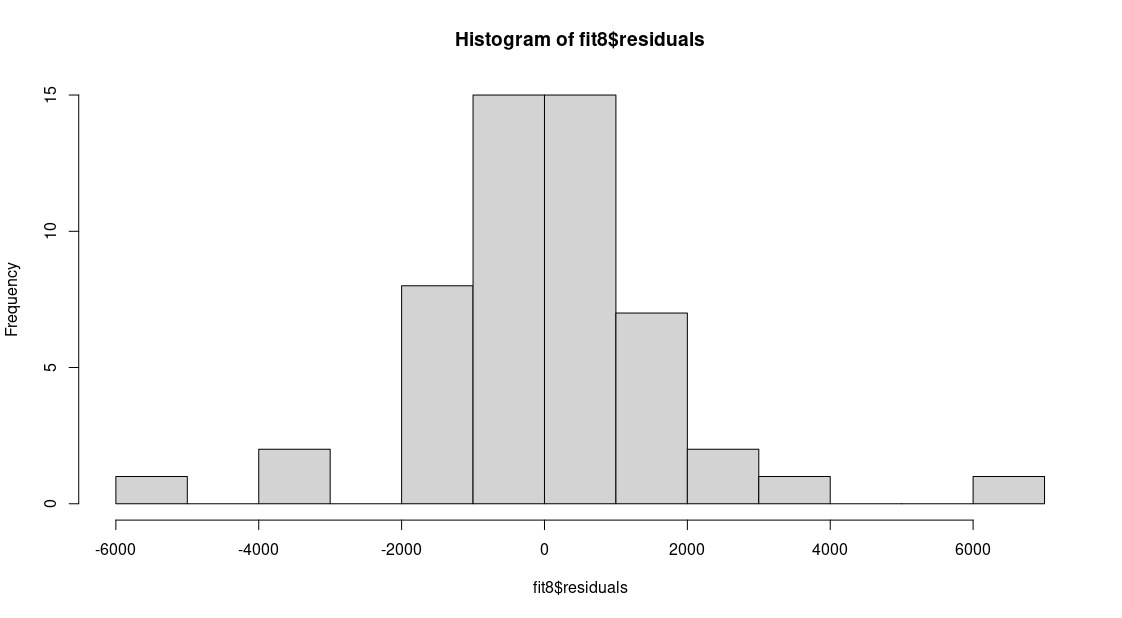
\includegraphics[scale=.45]{fit8residualsHist.PNG}
    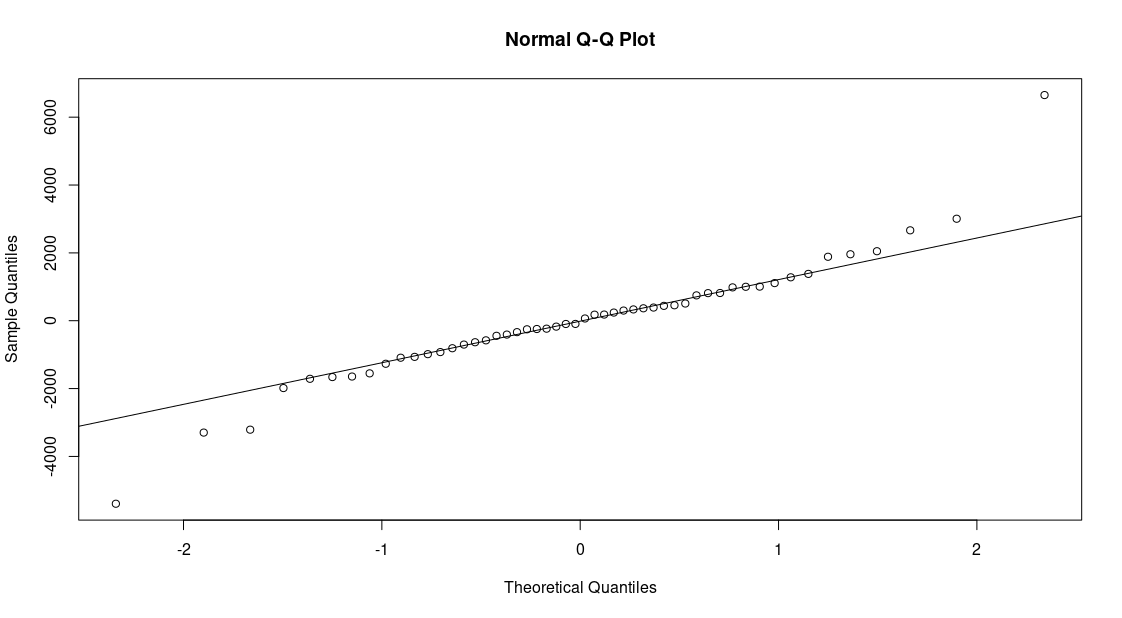
\includegraphics[scale=.45]{fit8ResidQQ.PNG}
  \end{center}
  \begin{verbatim}
# ongetransformeerde model:
fit8 = lm(formula = sales ~ assets + marketval + sector + sector:assets + sector:marketval)

# De verdeling van de residuen:
# extended KS-test voor normaliteit:
T_KS_8 = ks.test((fit8$residuals - mean(fit8$residuals))/sd(fit8$residuals), pnorm)$statistic

> pvalue(T_KS_8)
[1] 0.01229
  \end{verbatim}
  \end{figure}
  
  Als we vervolgens ook nog een aangepaste KS-toets uitvoeren (met de functies en simulatieverdeling als onder \ref{KS-toets}), dan verwerpen we met een $p$-waarde van 0.012 $<$ 0.05 dat de residuen normaal verdeeld zijn.
  
  Een mogelijke verklaring is dat de errors een \emph{mix van normale verdelingen} afkomstig zijn, namelijk per sector is er een `eigen verdeling' voor de errors die voor elke sector mean 0 maar een andere variantie heeft.
  
\section{Economische interpretatie}
  Deze verklaring is economisch te interpreteren als: in verschillende sectoren is er verschillende onzekerheid over de mate waarin ons model verklarend is. Sommige sectoren gedragen zich `netjes' ten opzichte van het model: daar zijn marktwaarde en kapitaal sterk verklarend voor de omzet, onze voorspelling wijkt daar meestal niet veel af van de werkelijkheid. Manufacturing zou dit bijvoorbeeld kunnen zijn. Andere sectoren zijn heel `wild': gegeven de marktwaarde en het kapitaal kunnen we eigenlijk niet veel zeggen over de omzet. Een voorbeeld van zo'n sector is misschien wel Energy.
  
\section{Herformulering Model}
\label{herformulering}
  
  We gaan het model herformuleren en dan binnen dit nieuwe model een toets formuleren: Blijkbaar moeten we de variantie $\sigma^2$ niet meer als \' e\' en uniforme parameter voor het hele model zien, maar als zijnde 4 individuele parameters van de submodellen. Het model ziet er dan als volgt uit:
  
  \begin{align}
  Y &= \begin{pmatrix} X_{\text{m}}  \\ X_{\text{f}} \\ X_{\text{r}} \\ X_{\text{e}} \end{pmatrix}\beta + \varepsilon \\
  \varepsilon &\sim \mathcal{N}(0,
  \begin{pmatrix} 
  \sigma_{\text{m}}^2I & & & \\ 
  & \sigma_{\text{f}}^2I & & \\ 
  & & \sigma_{\text{r}}^2I & \\
  & & & \sigma_{\text{e}}^2I \\
  \end{pmatrix})
  \end{align}
  
  Waarbij de blokken $X_{\text{s}}$ steeds de rijen van de designmatrix bevatten die datapunten bevatten uit sector s.
  
\section{Toetsen}

  We kunnen het bovenstaande vermoeden proberen te toetsen. De hypothesen zijn:
  \begin{align}
  H_0&: \sigma_1=\sigma_2=\sigma_3=\sigma_4 & H_1&: \sigma_1
  \neq \sigma_2 \neq \sigma_3 \neq \sigma_4
  \end{align}
  
  Waarbij we de levels van sector even nummeren in plaats van ze bij naam te noemen. We houden de nummering aan die \verb!R! hanteert, vraag deze eventueel op met \verb!levels(sector)!.
  
  Om de hypothese te toetsen is een kritiek gebied nodig. Als hulp is in de opgave een toetsingsstatistiek gegeven, namelijk 
  
  \begin{equation*}
    T = (n-k)\log(\frac{SS_{\text{res}}}{n-k}) - \sum_{i=1}^4 (n_i-k_i)\log(\frac{SS_{\text{res}}^{(i)}}{n_i-k_i})
  \end{equation*}
  
  Hierbij is $n$ de steekproefomvang, $k$ het totaal aantal regressieparameters, $n_i$ de grootte van het blok van de steekproef dat in categorie $i$ valt en $k_i$ het aantal parameters voor categorie $i$.
  
  We willen de nulverdeling van deze statistiek weten om hieruit de kritieke waarden te kunnen afleiden. Simulatie is hier de natuurlijke benadering. De verdelingen van $SS_{\text{res}}^{(i)}$ zijn namelijk:
  
  \begin{align*}
  \frac{SS_{\text{res}}^{(i)}}{\sigma_i^2} \sim \chi_{n_i-k_i}^2
  \end{align*}
  
  Waarbij de residuen van verschillende categorie\"en niet overlappen en dus niets met elkaar te maken hebben, oftewel onafhankelijk verdeeld zijn. Daardoor zijn de residuele kwadraatsommen van verschillende categorie\"en ook onafhankelijk. En $SS_{\text{res}} = \sum_{i=1}^4 SS_{\text{res}}^{(i)}$, is simpelweg de som van alle residuele kwadraatsommen (dus ook volledig \emph{afhankelijk} van die laatse). Onder de nulhypothese zijn de $\sigma_i^2$ aan elkaar gelijk, namelijk $\sigma^2$.
  
  We zien echter dat de nulhypothese samengesteld is: hij hangt namelijk nog af van $\sigma$, en vormt dus een eendimensionale deelruimte van de vierdimensionale parameterruimte voor de mogelijke varianties. Dit maakt simulatie niet direct triviaal, want misschien hangt de nulverdeling van $T$ dus nog af van de ware parameter (van welk punt van de nulhypothese we kiezen). We zullen op een of andere manier moeten aantonen dat het niet uitmaakt met welke $\sigma$ onze simulatiegrootheden geschaald worden.
  
  We gaan dit aantonen met de volgende berekening: zij steeds $Y_i \sim \chi_{n_i-k_i}^2$, Dan geldt onder $H_0$:
  
  \begin{align*}
    T &\sim (n-k)\log\left(\frac{\sigma^2(Y_1+Y_2+Y_2+Y_4)}{n-k}\right) - \sum_{i=1}^4 (n_i-k_i)\log\left(\frac{\sigma^2Y_i}{n_i-k_i}\right) \\
    &= (n-k)(\log(\sigma^2) +\log\left(\frac{(Y_1+Y_2+Y_2+Y_4)}{n-k}\right) ) - \sum_{i=1}^4 (n_i-k_i)(\log(\sigma^2)+\log\left(\frac{Y_i}{n_i-k_i}\right) ) \\
    &= (n-k)\log(\sigma^2) - \sum_{i=1}^4 (n_i-k_i)\log(\sigma^2) \\
     &\quad + (n-k)\log\left(\frac{Y_1+Y_2+Y_2+Y_4}{n-k}\right) - \sum_{i=1}^4 (n_i-k_i)\log\left(\frac{Y_i}{n_i-k_i}\right) \\
  \end{align*}
  
  Met $(n-k) = \sum_{i=1}^4 n_i - \sum_{i=1}^4 k_i = \sum_{i=1}^4 (n_i-k_i)$ volgt nu dat de voorste term `$(n-k)\log(\sigma^2) - \sum_{i=1}^4 (n_i-k_i)\log(\sigma^2)$' wegvalt, en we houden over:
  \begin{equation}
  T \sim (n-k)\log\left(\frac{Y_1+Y_2+Y_2+Y_4}{n-k}\right) - \sum_{i=1}^4 (n_i-k_i)\log\left(\frac{Y_i}{n_i-k_i}\right)
  \end{equation}
  Wat niet meer afhangt van enige onbekende parameter. We kunnen deze statistiek onder $H_0$ dus gewoon simuleren in \verb!R! met behulp van chikwadraat-verdelingen. We simuleren namelijk steeds 
  \begin{align*}
  Y_i &\sim \chi^2_{n_i-k_i} \\
  Y &\leftarrow \sum_{i=1}^4 Y_i
  T &\leftarrow (n-k)\log\left(\frac{Y}{n-k}\right) - \sum_{i=1}^4 (n_i-k_i)\log\left(\frac{Y_i}{n_i-k_i}\right)
  \end{align*}
   
  De constantes $n,k,n_i,k_i$ kunnen we allemaal in \verb!R! opvragen en ga ik hier niet onnodig opschrijven.
  
\section{Simulatie van $T$ en conclusie}
  Het volgende \verb!R!-script is gebruikt om $T$ te simuleren en een histogram te maken van de nulverdeling:
  
  \begin{figure}[H]
  \begin{verbatim}
# Simulatie van de statistiek T:
# eerst de aantallen:
n = 52 #steekproefgrootte
k = 12 #regressieparameters totaal

SSres = sum(fit8$residuals^2) #totale residuele kwadratensom

k_ = c(3,3,3,3) #vector met per index i aantal parameters van submodel (=3)
n_ = numeric(4) #vector waarin steekproefgrootte per submodel komt
SSres_ = numeric(4) #vector waarin SSres(i) per submodel komt

for (l in 1:nlevels(sector)){ #vraag per submodel steekproefgrootte n_ en SSres_ op
  n_[l] = sum(as.numeric(sector) == l)
  SSres_[l] = sum(fit8$residuals[which(as.numeric(sector) == l)]^2)
}

TestStatistic = (n-k)*log(SSres/(n-k)) - sum((n_-k_)*log(SSres_/(n_-k_)))

SimT_ = numeric(N) # N is een constante, aantal simulaties (ergens hierboven gedefinieerd = 10000)
for (i in 1:N){
  X = numeric(4)
  for (l in 1:4){
    X[l] = rchisq(1,df = n_[l] - k_[l]) #simuleer uit chisquare n_i-k_i
  }
  SimT_[i] = (n-k)*log(sum(X)/(n-k)) - sum((n_-k_)*log(X/(n_-k_)))
}

hist( D
    , probability = TRUE
    , breaks = 100
    , main = "Histogram van de nulverdeling van T"
    , xlab = "T"
    , ylab = "dichtheid")

lines(c(TestStatistic,TestStatistic), c(0,N), lwd = 2, col = "blue") 
  \end{verbatim}
  \end{figure}
  
  Dit produceert de volgende nulverdeling:
  \begin{figure}[H]
  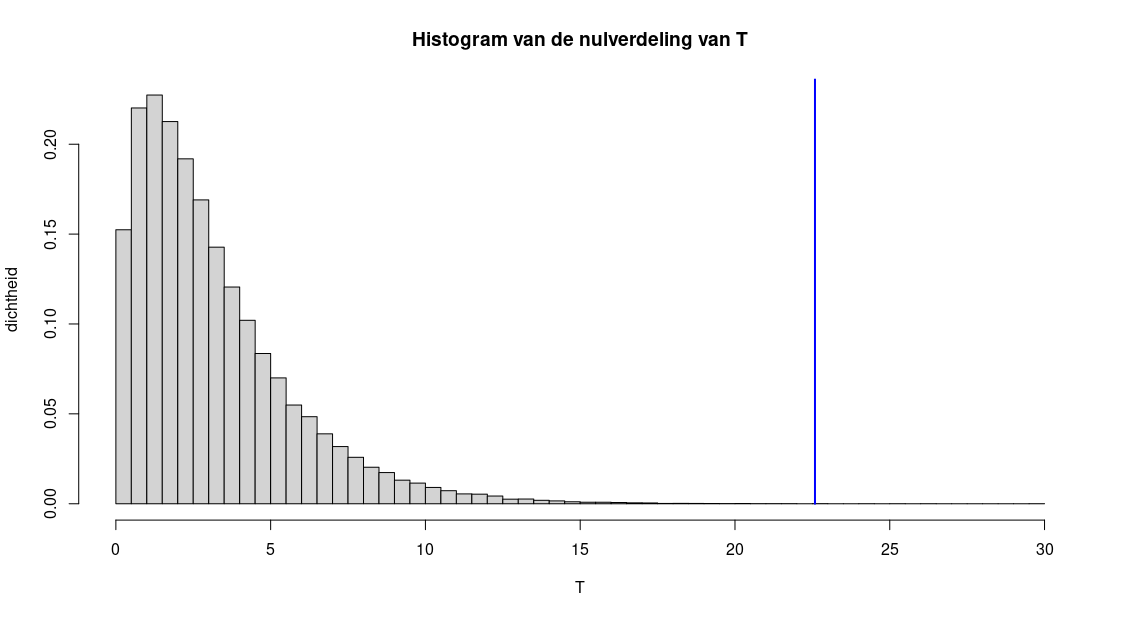
\includegraphics[scale= 0.45]{NullTpart6.png}
  \end{figure}
  
  En het berekenen van een $p$-waarde is nu eenvoudig:
  \begin{verbatim}
> pval = mean(SimT_ > TestStatistic) 
> pval
[1] 5e-05
  \end{verbatim}
  
  We concluderen dat de varianties verschillen tussen de sectoren. Dit zegt nog niet welke sectoren grotere/kleinere varianties hebben, maar wel dat er verschil is.
  
\section{Problemen voor het schatten?}
  De vraag is nu of onze schattingsprocedure voor de regressieparameters in het oude model dan wel zuiver of effici\"ent genoeg waren onder de modelaanname dat de varianties inderdaad verschillen per sector. 
  
  Andere varianties per submodel maakt echter niets uit voor de kleinste-kwadratenschatter. Deze schat immers de regressieparameters per submodel (dus per sector $i$ onafhankelijk) van de andere submodellen (die een 0 in die kolom hebben). Daardoor is de variantie binnen het submodel waarbinnen we schatten nog steeds \' e\' en constante, en hoeven er geen aanpassingen zoals weighted least squares te worden toegepast.
  
\section{Welke sector heeft de grootste variantie?}
  Deze vraag kunnen we proberen te beantwoorden door naar de $\frac{SS_{\text{res}}^{(i)}}{n_i-k_i}$'s te kijken. Deze vormen immers zuivere schatters voor de varianties:
  
  \begin{verbatim}
> levels(sector)
[1] "Energy"        "Finance"       "Manufacturing" "Retail"       
> SSres_/(n_-k_)
[1]  1115843  1109813  4812990 13382743 
  \end{verbatim}
  
  We zien dat Retail en daarna Manufacturing heel grote varianties hebben, terwijl Energy en Finance kleinere schattingen hebben en deze ook redelijk dicht bij elkaar liggen.
  
  Dit betekent dus dat ons model betere voorspellingen kan doen in die laatste twee sectoren dan in de eerste twee. Hoeveel beter zou je weer verder kunnen kwantificeren.
  
\section{Waarom deze toets eigenlijk niet valide is}
  De bovenstaande toetsingsstatistiek heeft onder de nulhypothese een verdeling die alleen afhangt van chikwadraatverdelingen, en hiermee hebben we de kritieke waarden bepaald. 
  
  Het model met aparte varianties per groep, wat wij hebben gerechtvaardigd met deze toets, neemt echter nog steeds aan dat de residuen normaal verdeeld zijn met verwachting 0 (waarbij nu de variantie van de residuen per sector een eigen parameter is). We kunnen echter met een aanpassingstoets laten zien dat deze aanname nog steeds niet overeenstemt met de werkelijkheid. Gebruiken we namelijk een KS-toets die toets of per sector de residuen normaal verdeeld zijn, dan verwerpen we voor twee sectoren (Finance en Retail) en voor \' e\' en sector bijna (Manufacturing) dat de residuen een normale verdeling volgen:
  
  \begin{figure}[H]
  \begin{verbatim}
T_KS_8_ = numeric(4)
for (i in 1:nlevels(sector)){
  # Bereken de KS-statistiek (ingebouwd in R)
  T_KS_8_[i] = ks.test((fit8$residuals[which(as.numeric(sector) == i)] 
                        - mean(fit8$residuals[which(as.numeric(sector) == i)]))
                       /sd(fit8$residuals[which(as.numeric(sector) == i)]), pnorm)$statistic
} 

# Bereken nu middels onze gesimuleerde nul-verdeling
# de p-waarde voor de extended ks-toets:

> pvalue(T_KS_8_[1]) # Energy
[1] 0.42299
> pvalue(T_KS_8_[2]) # Finance
[1] 0.0016
> pvalue(T_KS_8_[3]) # Manufacturing
[1] 0.05621
> pvalue(T_KS_8_[4]) # Retail
[1] 0.00064
  \end{verbatim}
  \end{figure}
  
  Om die reden kun je je afvragen in hoeverre het verwerpen van $$H_0: \sigma_1 = \sigma_2 = \sigma_3 = \sigma_4$$ het model uit \ref{herformulering} rechtvaardigt. We moeten in ieder geval beseffen dat het verwerpen van $H_0$ en het accepteren van het model uit \ref{herformulering} twee drastische verschillende dingen zijn!
  
  Bovendien kan het uitvoeren van de toets met toetsingsstatistiek $T$ dus ook tot type II fouten leiden: in het geval dat de varianties van de residuen wel sterk verschillen tussen de groepen maar er geen normale verdeling gevolgd wordt, zodat de uiteindelijke waarde van $T$ voor de data niet heel incompatibel is met de nulhypothese. De nulhypothese gaat namelijk wel uit van normaal verdeelde residuen (we simuleren de $SS_{\text{res}}^{(i)}$ per slot van rekening uit chikwadraatverdelingen!), terwijl hier helemaal geen sprake van is.
  
  Dit laat zien dat toetsen eigenlijk slechts valide zijn binnen een bepaald model. Als de werkelijke data het model niet volgt, moeten we ons afvragen of toetsen bijvoorbeeld niet te sterk worden. We hebben de toets met $T$ in het voorgaande deels gerechtvaardigd door te verondstellen dat de residuen een mixverdeling van 4 normale verdelingen volgden, en deze hypothese werd in deze sectie juist verworpen. 
  
  Misschien is het daarom beter om de toets zelf ook maar niet te veel autoriteit te geven, en te zeggen dat we niet weten of de varianties werkelijk verschillen. Het enige wat we met zekerheid kunnen zeggen is dat er modelaannames uit zowel \ref{Model} als uit \ref{herformulering} door deze fit geschonden worden (dit blijkt namelijk uit de aanpassingstoetsen).
  
\chapter{Assimileren van de levels van sector in \ref{uitbreiding logmarketval:sector}}

  We zagen in \ref{uitbreiding logmarketval:sector} dat het toevoegen van interactieterm \verb!logmarketval:sector! door de $F$-toets niet gerechtvaardigd kon worden (we konden de hypothese dat alle toegevoegde parameters nul waren, niet verwerpen bij significantie 0.05). Toch was de overschrijdingskans, hoewel te hoog, nog redelijk laag: waar deze in \ref{uitbreiding logassets:sector} 0.74 was, was deze voor \ref{uitbreiding logmarketval:sector} slechts 0.15. 

  Bovendien zien we in de summary van \ref{uitbreiding logmarketval:sector} dat met name \verb!logmarketval:sectorRetail! een heel zinloze variabele is, met een effect dat wel erg dicht bij 0 ligt.
  
  Een `fix' hiervoor is om Retail en Energy te `mergen' tot \' e\' en level van sector. Sector heeft dan nog maar 3 levels. Dit reduceert het aantal toegevoegde parameters als we interactietermen toevoegen aan model \ref{Basale Model}, wat mogelijk leidt tot verbetering.
  
\section{Rechtvaardiging van het idee}

  Dit idee is niet geheel onomstreden. Immers, waarom zou het zinnig zijn om twee verschillende sectoren als dezelfde sector te beschouwen? Welke interpretatie heeft dit eigenlijk?
  
  Ik wil het volgende voorbeeld geven om het idee enigszins natuurlijk te doen overkomen. 
  
  Stel, een bioloog verzamelt data over schutkleuren bij vissen. Hij zet gele, magenta, cyane, mosgroene en bruine vissen uit in de natuur en, weet ik veel, hij schat een survivalmodel of iets dergelijks, met als verklarende variabele de kleur (categorisch met de hiervoor genoemde levels). Wat blijkt, met geel als base-level blijken cyaan en magenta niet significant. Met mosgroen als base-level blijkt bruin niet significant. Misschien wordt met de $F$-toets de nulhypothese van geen totaal effect nog wel verworpen, maar als we maar genoeg verschillende kleurenlevels defini\"eren groeit het aantal parameters $p$ vanzelf tot een grootte waar dat ook niet meer gebeurt.
  
  In werkelijkheid begrijpen we prima wat er aan de hand is en wat we willen aantonen, namelijk dat felgekleurde vissen minder lang overleven in een natuurlijke omgeving. Waarom `assimileren' de levels niet tot de twee levels `felgekleurd' en `donkergekleurd', die zeker wel verschillende effecten zullen hebben? Je hoeft dan slechts twee parameters te schatten, wat de variantie van het schatten kleiner maakt, en indien er inderdaad zo'n effect is ook nog zuiver.
  
  Hetzelfde stellen we nu voor bij de levels: door Energy en Retail samen te voegen in de interactieterm bedoelen we niet dat dit geen verschillende sectoren zijn, maar eerder dat de twee groepen bedrijven op bepaalde vlakken zodanig overeenkomstig zijn dat het zinloos is ze een eigen effect toe te kennen. Net zoals we vissenkleuren echt heel mooi en heel verschillend vinden, maar we toch ook kunnen spreken over `felgekleurd' en `donkergekleurd'
  
  Natuurlijk is alles relatief. Het vissen-voorbeeld is dan ook een situatie waarin merging van levels een logische keuze is. In het onderstaande zullen we echter zien dat we het model verklarender kunnen maken met een heel onnatuurlijke assimilatie. De vraag wordt dan natuurlijk of we echt met zo'n model willen werken, of dat we aan het overfitten zijn.
  
\section{Implementatie}
  Je kunt in \verb!R! als volgt levels aanpassen:
  
\begin{verbatim}

mergesector <- sector

levels(mergesector)[levels(mergesector) == "Energy"] <- "Merge"
levels(mergesector)[levels(mergesector) == "Retail"] <- "Merge"

fitMerge = lm(formula = logsales ~ logassets + logmarketval + sector + logmarketval:mergesector)
\end{verbatim}

  \verb!fitMerge! heeft de volgende ANOVA-table (waarin we dus de $F$-toets kunnen aflezen):
  
  
\begin{verbatim}
Analysis of Variance Table

Response: logsales
                         Df  Sum Sq Mean Sq F value    Pr(>F)    
logassets                 1  9.4344  9.4344 36.0221 3.354e-07 ***
logmarketval              1 23.5890 23.5890 90.0666 3.270e-12 ***
sector                    3 24.5162  8.1721 31.2023 5.722e-11 ***
logmarketval:mergesector  2  1.5289  0.7645  2.9188   0.06452 .  
Residuals                44 11.5239  0.2619                      
---
Signif. codes:  0 ‘***’ 0.001 ‘**’ 0.01 ‘*’ 0.05 ‘.’ 0.1 ‘ ’ 1
\end{verbatim}

  Helaas, het werkt n\' et niet. We verwerpen de $F$-toets niet, maar slechts op 1\% na. Dit zijn overigens de geschatte regressieparameters:
  
\begin{verbatim}
Coefficients:
                                      Estimate Std. Error t value Pr(>|t|)    
(Intercept)                            0.85493    0.96069   0.890   0.3784    
logassets                              0.62181    0.08888   6.996 1.16e-08 ***
logmarketval                           0.21794    0.15155   1.438   0.1575    
sectorFinance                         -2.42445    1.23803  -1.958   0.0566 .  
sectorManufacturing                    2.35453    1.38601   1.699   0.0964 .  
sectorRetail                           1.37674    0.21882   6.292 1.26e-07 ***
logmarketval:mergesectorFinance        0.24333    0.18297   1.330   0.1904    
logmarketval:mergesectorManufacturing -0.20777    0.19850  -1.047   0.3010    
\end{verbatim}
  

  Nu wil ik iets interessants laten zien. Je denkt nu namelijk vast: wat flauw, om het aantal levels maar zodanig te reduceren dat er vanzelf wel iets significant wordt. Stel bijvoorbeeld dat we ook Manufacturing, de variabele met de estimate die nu het dichtst bij 0 ligt, ook zouden assimileren in \verb!Merge!.
  
\begin{verbatim}
Residuals:
     Min       1Q   Median       3Q      Max 
-0.81188 -0.35962 -0.09961  0.30965  1.15602 

Coefficients:
                               Estimate Std. Error t value Pr(>|t|)    
(Intercept)                     0.91635    1.00952   0.908    0.369    
logassets                       0.59803    0.09285   6.441 6.90e-08 ***
logmarketval                    0.23656    0.15910   1.487    0.144    
sectorFinance                  -1.23163    1.19124  -1.034    0.307    
sectorManufacturing             0.52743    1.21591   0.434    0.667    
sectorRetail                    1.36194    0.22993   5.923 4.06e-07 ***
logmarketval:mergesectorMerge2  0.05538    0.17371   0.319    0.751    
---
Signif. codes:  0 ‘***’ 0.001 ‘**’ 0.01 ‘*’ 0.05 ‘.’ 0.1 ‘ ’ 1

Residual standard error: 0.538 on 45 degrees of freedom
Multiple R-squared:  0.8155,	Adjusted R-squared:  0.7909 
F-statistic: 33.15 on 6 and 45 DF,  p-value: 5.952e-15
\end{verbatim}

\begin{verbatim}
Analysis of Variance Table

Response: logsales
                         Df  Sum Sq Mean Sq F value    Pr(>F)    
logassets                 1  9.4344  9.4344 35.9458 3.171e-07 ***
logmarketval              1 23.5890 23.5890 89.8758 2.694e-12 ***
sector                    3 24.5162  8.1721 31.1362 4.740e-11 ***
logmarketval:mergesector  1  1.2420  1.2420  4.7321    0.0349 *  
Residuals                45 11.8108  0.2625                      
---
Signif. codes:  0 ‘***’ 0.001 ‘**’ 0.01 ‘*’ 0.05 ‘.’ 0.1 ‘ ’ 1
\end{verbatim}

  
  Ik denk dat dit voorbeeld goed weergeeft dat niet elk model dat door toetsen heenkomt en een grotere verklarende waarde heeft op een sample ook daadwerkelijk een zinnig model is waarmee men in de werkelijkheid voorspellingen wil doen. De $F$-toets verwerpt de nulhypothese van geen verklarende waarde. Maar in werkelijkheid hebben we net zolang sectoren samengeveegd totdat er \' e\' en was (namelijk "Manufacturing, maar ik geloof dat we hetzelfde voor "Finance" zouden kunnen doen) die voldoende afwijkende datapunten had om als regressor significant te zijn.
  
  Ik zou het bovenstaande model nooit beter noemen dan het basale model \ref{Basale Model}. Ik denk dat dit model simpelweg een geval van overfitting is die zich bij de huidige steekproefgrootte door de standaardtoetsen weet te wurmen.
  
\chapter{Conclusie}

  Het uiteindelijke `beste' model bleek gewoon het basismodel met 6 parameters te zijn. Zoals al het vermoeden was bij het zien van de 2d-plots van de data, was een logtransformatie nodig om de heteroskedasticiteit uit de data te halen.
  
  Deze logtransformatie legde tevens een mooie clustering van de data bloot in het scatterplot van \verb!logsales! tegen \verb!logassets!: de data uit verschillende sectoren vormde samen een wanordelijke wolk, maar met kleuring van de levels werd zichtbaar dat de punten per sector eigenlijk keurig rond een familie van boven elkaar liggende bijna-parallelle lijnen lagen. Dit maakte de opname van de categorische variabele \verb!sector! in het model tot natuurlijke keuze. 
  
  Het basismodel bleek inderdaad goed te verklaren. De continue variabelen waren individueel significant volgens de default $t$-toetsen in de summary door \verb!R!. \verb!sector! kon na de uitvoer van een $F$-toets ook bijzonder significant worden genoemd.
  
  Uitbreidingen op het model met interactietermen bleken weinig succesvol: de nulhypothese van geen effect kon in geen van de drie voorgestelde uitbreidingen worden verworpen. 
  
  Ook hebben we gekeken naar een model zonder de logtransformaties, in welk geval de uitbreiding met alle interactietermen door alle $F$-toetsen bleek te komen (ditmaal ontdekten we dat niet na 10 regels script, maar met een snelle blik op de ANOVA-table).
  
  In feite was dit model een collectie van 4 losse modellen (er waren geen gedeelde hoofdeffecten), en daardoor werd het mogelijk om de varianties per submodel te schatten en middels een toetsingsstatistiek $T$ te bepalen of er misschien geen sprake was van groepsheteroskedasticiteit. De nulhypothese van homoskedasticiteit werd inderdaad verworpen. 
  
  We kunnen echter met zekerheid zeggen dat het model waarbinnen deze toets geconstrueerd is, waarschijnlijk niet het werkelijke model is dat de data volgt (aangezien de residuen per sector nog steeds niet normaal verdeeld waren, aldus de KS-aanpassingstoets). Daarom is de validiteit van deze toets in twijfel te trekken.
  
  In het laatste hoofdstuk hebben we met de beste bedoelingen geprobeerd om sectoren te assimileren, zodat we minder parameters hoeven te schatten in mogelijke uitbreidingen op het 6-parametermodel, maar uiteindelijk is dit pad weer verlaten nadat het eigenlijk geen zinvolle interpretatie meer bleek te hebben.

  Het grote ongetransformeerde model en het basale 6-parametermodel zijn als beste uit de bus gekomen. Hiervan verklaart het 6-parametermodel eigenlijk even goed, met de helft van de parameters van het grote model. Daarnaast is onder \ref{economische motivatie} besproken dat een $\log$-transformatie de economische werkelijkheid beter weerspiegelt. Al met al is de keuze toch gevallen op het eenvoudigste, haast na\"ieve model.
  
  Hiermee kunnen nu voorspellingen worden gedaan over de omzetten van grote bedrijven, wanneer we de marktwaarde, sector en het kapitaal kunnen achterhalen. Uiteraard moet rekening worden gehouden met selectievertekening (we hebben een model gefit op de 52 grootste bedrijven, niet op een aselecte steekproef uit alle bedrijven) en het bestaan van andere, onbekende sectoren. We hopen maar dat dit het businessplan ten goede komt...
\end{document}
